% @Author: Taha Bouhsine

%%%%%%%%%%%%%%%%%%%%%%%%%%%%%%%%%%%%%%%%%%%%%%%%%%%%%%%%%%%%%%%%%%%%%%%%%%%
% This is the main file
% You can add/remove chapters/pdf files here
%%%%%%%%%%%%%%%%%%%%%%%%%%%%%%%%%%%%%%%%%%%%%%%%%%%%%%%%%%%%%%%%%%%%%%%%%%%

\documentclass[12pt, oneside, a4paper]{fsa-pfe-report}

%%%%%%%%%%%%%%%%%%%%%%%%%%%%%%%%%%%%%%%%%%%%%%%%%%%%%%%%%%%
% Define code variables
%%%%%%%%%%%%%%%%%%%%%%%%%%%%%%%%%%%%%%%%%%%%%%%%%%%%%%%%%%%
\graphicspath{{images/}}

%%%%%%%%%%%%%%%%%%%%%%%%%%%%%%%%%%%%%%%%%%%%%%%%%%%%%%%%%%%
%% Include required packages
%%%%%%%%%%%%%%%%%%%%%%%%%%%%%%%%%%%%%%%%%%%%%%%%%%%%%%%%%%%
%\usepackage{showframe}

\usepackage[skins]{tcolorbox}
\usepackage[francais,english]{babel}
\usepackage[english]{varioref}
\usepackage[export]{adjustbox}
\usepackage{acro}
\usepackage{setspace}
% \usepackage{minted}
\usepackage{color}
\usepackage{tabularx}
\usepackage{ctable}
\usepackage{graphicx}
\usepackage{multirow}
\usepackage{tikz}
\usepackage{seqsplit}
\usepackage{fontenc}
%\usepackage{lipsum}
%\usepackage{todonotes}
\usepackage{wrapfig}
\usepackage{setspace}
\usepackage[all]{nowidow}

\usepackage[sorting=none, backend=bibtex]{biblatex}
\addbibresource{001-report}

%% TODO: Remove this function when done %%
\newcommand\todoin[2][]{\todo[inline, caption={2do}, #1]{
\begin{minipage}{\textwidth-4pt}#2\end{minipage}}}

%%%%%%%%%%%%%%%%%%%%%%%%%%%%%%%%%%%%%%%%%%%%%%%%%%%%%%%%%%%
% Include useful commands
%%%%%%%%%%%%%%%%%%%%%%%%%%%%%%%%%%%%%%%%%%%%%%%%%%%%%%%%%%%
% @Author: Taha Bouhsine
% @Date:   17-03-2020

%%%%%%%%%%%%%%%%%%%%%%%%%%%%%%%%%%%%%%%%%%%%%%%%%%%%%%%%%%%%%%%%%%%%%%%%%%%
% In this file, you will put the details of your graduation project
%%%%%%%%%%%%%%%%%%%%%%%%%%%%%%%%%%%%%%%%%%%%%%%%%%%%%%%%%%%%%%%%%%%%%%%%%%%

\newcommand{\reportTitle} {%
  \textsc{PROJECT DE FIN D'ÉTUDE}%
}

\newcommand{\reportAuthor} {%
  Taha \textsc{Bouhsine}%
}

\newcommand{\reportSubject} {%
  Design And Full Stack Development Of A Crowdfunding Platform \\ Sahem %\\ %With MongoDB, Express JS, Angular 9 And NodeJs%
}

\newcommand{\dateSoutenance} {%
  25/5/2020%
}

\newcommand{\studyDepartment} {%
  Département d'Informatique%
}
\newcommand{\filiere}{
  Filière Sciences Mathématiques et Informatique
}

\newcommand{\FSA} {%
  Faculté des Sciences Agadir%
}
\newcommand{\UIZ}{
  UNIVERSITÉ IBN ZOHR
}

\newcommand{\codePFE} {% Reference
  FSA-PFE-001%
}
\newcommand{\mentor}{
  Dr. \textsc{BELAQZIZ Salwa}
}
\newcommand{\juryPresident} {%
  Mr Foulen \textsc{Fouleni}%
}
\newcommand{\juryPresidentDesc} {%
  President%
}

\newcommand{\juryMemberOne} {%
  Ms Jury \textsc{One}%
}
\newcommand{\juryMemberOneDesc} {%
  Supervisor %Mentor
}

\newcommand{\juryMemberTwo} {%
  Mr Jury \textsc{Two}%
}
\newcommand{\juryMemberTwoDesc} {%
  Reviewer% Examiner, Reporter
}

\newcommand{\specialcell}[1]{%
  \begin{tabularx}{\textwidth}{@{}X@{}}#1\end{tabularx}%
}

%%%%%%%%%%%%%%%%%%%%%%%%%%%%%%%%%%%%%%%%%%%%%%%%%%%%%%%
% Add your own commands here
%%%%%%%%%%%%%%%%%%%%%%%%%%%%%%%%%%%%%%%%%%%%%%%%%%%%%%%
\newcommand{\latex}{\LaTeX\xspace}
\newcommand{\tex}{\TeX\xspace}

%%%%%%%%%%%%%%%%%%%%%%%%%%%%%%%%%%%%%%%%%%%%%%%%%%%%%%%
% Add your own acronyms here
%%%%%%%%%%%%%%%%%%%%%%%%%%%%%%%%%%%%%%%%%%%%%%%%%%%%%%%
\DeclareAcronym{SMI}{%
  short=SMI,%
  long=Sciences Mathématiques et Informatique%
}
\DeclareAcronym{FSA}{
  short=FSA,
  long=Faculté des Sciences Agadir
}

\hypersetup{
  pdftitle={\reportTitle~-~\reportSubject},%
  pdfauthor={\reportAuthor},%
  pdfsubject={\reportSubject},%
  pdfkeywords={report} {crowdfunding} {pfe} {fsa}
}

\begin{document}
  \begin{pfe-fsa}
    \pagenumbering{roman}% i ii iii iv ...

    % \listoftodos{}

    % Front matter
    % @Author: Taha Bouhsine

%%%%%%%%%%%%%%%%%%%%%%%%%%%%%%%%%%%%%%%%%%%%%%%
% Only edit this file for fine tuning to your own needs/liking
% There isn't really much to edit here
%%%%%%%%%%%%%%%%%%%%%%%%%%%%%%%%%%%%%%%%%%%%%%%

\thispagestyle{empty}

% after Soutnence
% \begin{titlepage}
%   \begin{sffamily}
%     \begin{center}

%       % Upper part of the page. The '~' is needed because \\
%       % only works if a paragraph has started.
%       \textsc{
%         \Large \bfseries \UIZ{}\\
%       }
%       \textsc{
%         \FSA{}\\[0.7cm]
%       }
%       
\includegraphics[scale=0.2]{assets/fsa.png}~\\[0.7cm]
%       \textsc{
%         \studyDepartment{}\\[0.7cm]
%       }
%       \textsc{
%         \reportTitle{}\\[0.7cm]
%       }
%       \begin{minipage}{0.5\textwidth}
%         \begin{center} \normalsize
%           \emph{Présenté Par:}
%           \textsc{
%             \reportAuthor{}
%           }\\[0.7cm]

%         \end{center}
%       \end{minipage}

%       \textsc{ Pour l’obtention de la \\
%         \large Licence en Sciences Mathématiques et Informatique }\\[1.5cm]

%       % Title
%       \HRule \\[0.4cm]
%       { \huge \bfseries \reportSubject \\[0.4cm] }

%       \HRule \\[2cm]
%       % Author and supervisor
%       \begin{minipage}{0.6\textwidth}
%         \begin{flushleft} \large
%           \emph{Encadré par : } \encadrent{} \\

%         \end{flushleft}
%       \end{minipage}
%       \newline \vskip1.5cm

%       Soutenu le \dateSoutenance, devant la commission d'examen:\\
%       \vspace{15pt}
%       \begin{tabular}{p{0.3\linewidth} p{0.15\linewidth}}
%         \juryPresident{} & \juryPresidentDesc{} \\
%         \juryMemberOne{} & \juryMemberOneDesc{} \\
%       \end{tabular}
%       \vskip1cm

%       \vfill

%       % Bottom of the page
%       {\large \emph{Année universitaire : } 2019 - 2020}

%     \end{center}
%   \end{sffamily}
%   \thispagestyle{empty}
% \end{titlepage}

\begin{titlepage}
  \begin{rmfamily}
    \begin{center}

      % Upper part of the page. The '~' is needed because \\
      % only works if a paragraph has started.

      
\includegraphics[scale=0.60]{assets/UIZ.jpg}~\\[0.7cm]
      \textsc{
        \Large \bfseries \UIZ{}\\
      }
      \textsc{
        \FSA{}\\[0.7cm]
      }

      \textsc{
        \Large \bfseries \studyDepartment{}\\[0.4cm]
      }
      \textsc{
        \large \filiere{}\\[0.7cm]
      }
      \textsc{
        \large \reportTitle{}\\[0.5cm]
      }
      \begin{minipage}{0.5\textwidth}
        \begin{center} \normalsize \bfseries
          \textsc{Présenté Par:}
          \textsc{
            \reportAuthor{}
          }\\[0.7cm]

        \end{center}
      \end{minipage}

      \textsc{ Pour l’obtention de la \\
        \bfseries \large Licence en Sciences Mathématiques et Informatique }\\[1cm]

      % Title
      \HRule \\[0.4cm]
      { \huge \bfseries \reportSubject \\[0.4cm] }

      \HRule \\[1cm]
      % Mentor
      \begin{minipage}{0.6\textwidth}
        \begin{flushleft} \large
          \textsc{Encadré par :} \mentor{} \\

        \end{flushleft}
      \end{minipage}
      \newline \vskip4cm


      \vfill

      % Bottom of the page
      {\large \emph{Année universitaire : } 2019 - 2020}

    \end{center}
  \end{rmfamily}
  \thispagestyle{empty}
\end{titlepage}

    \cleardoublepage%

    % @Author: Taha Bouhsine

\chapter*{Dedication}
\addcontentsline{toc}{chapter}{Dedication}
\thispagestyle{empty}
%
%For all they have endured to satisfy all my needs and wishes
\begin{center}
  In memoriam Hanya Laaiba, my dear grandmother, ~ \\
  her last words of encouragement are living with me to this day, ~ \\
  feeding my motivation, and always urging me to pursue my dreams, and my studies, ~\\
  never to be forgotten, never to be erased, ~ \\
  may your soul rest in peace, ~ \\
  may your memory guide me trough my future steps to the unknown ~ \\


\end{center}
%
\nopagebreak{%
  % And maybe a quote here
  \raggedright\hspace{5.75cm} To your beautiful soul,~\\
  \raggedright\hspace{7.75cm} I dedicate this work\@.~\\~\\~\\
  %
  \raggedleft\normalfont\large\itshape{} \reportAuthor\par%
}
%
%
%
%
%
%
\cleardoublepage%
\chapter*{Thanks}
\addcontentsline{toc}{chapter}{Thanks}
\thispagestyle{empty}
%
I wish to express my sincere appreciation to my supervisor, Doctor Belaqziz Salwa,
who has the substance of a genius: she convincingly guided and encouraged me to be
professional and do the right thing even when the road got tough. Without her
persistent help, the goal of this project would not have been realized.\\

I wish to acknowledge the help provided by the administration staff in
Ibn Zohr University, Faculty of Science, and would like to thank them for giving us a great studying
environment.
And to all our classmates and the professors of Computer Science Departement for having contributed
in the formulation of our ideas and for providing a suitable working environment towards the completion of
this project.\\

Finally, I must express my very profound gratitude to my parents and my friends
for providing me with unfailing support and continuous encouragement throughout my years
of study and through the process of researching and developing this project.
This accomplishment would not have been possible without them. Thank you.

\cleardoublepage%
\chapter*{Abstract}
\addcontentsline{toc}{chapter}{Abstract}
\thispagestyle{empty}
%
Crowdfunding refers to behavior where public individuals, rather than institutions, to use digital
technologies to make financial contributions to people, projects, or businesses in response to
either financial or developmental commitments from those people, projects, or businesses.
Sahem Crowdfunding Platform is a project that aims to develop a system that will be a gateway to allow project funders to
contribute towards a good project idea of a creator who lacks sufficient resources to implement
the project idea. It is important to develop this project because it will seek to create a platform
that will bridge the gap between viable project ideas and successful implementation of these
projects so that good project ideas that can benefit individuals and the community at large cannot
go into a waste.
With the aim to successfully develop this project, we will employ the use of the Software
development methodology, Iterations and Increments process, as well as we will be using the Kanban board Model
to divide and organize our project into, and also will be carrying out reviews and analysis of existing solutions in an attempt to
create a unique user experience with the use of Stripe API as payment.
    \cleardoublepage%

    \tableofcontents
    \addcontentsline{toc}{chapter}{\contentsname}
    \cleardoublepage%

    \listoffigures
    \addcontentsline{toc}{chapter}{\listfigurename}
    \cleardoublepage%

    \listoftables
    \addcontentsline{toc}{chapter}{\listtablename}
    \cleardoublepage

    %\printglossary[type=\acronymtype, title=Abbreviations]
    \printacronyms[heading=chapter*, name=Acronyms]
    \addcontentsline{toc}{chapter}{Acronyms}
    \cleardoublepage%

    \sloppy

    \pagenumbering{arabic}% 1 2 3 4 5
    \doublespacing{}% Double spacing between lines

    \addtocontents{toc}{\protect\setcounter{tocdepth}{2}}

    % Main matter
    % @Author: Taha Bouhsine


%%%%%%%%%%%%%%%%%%%%%%%%%%%%
% CHAPTER                  %
%%%%%%%%%%%%%%%%%%%%%%%%%%%%
\chapter*{Introduction}
\label{chap:general_intorduction}
\markboth{\MakeUppercase{Introduction}}{}%
\addcontentsline{toc}{chapter}{Introduction}%

One of the main reasons the humans survived through time 

\section*{ Project Presentation }
\subsection*{Problem}
\subsection*{Objectifs}
\subsection*{Document Organization}


\section*{Crowdfunding}
\subsection*{Definition}
\subsection*{History}
\subsection*{Principe / Functionality }
\subsection*{ Before Crowdfunding, the Peer-To-Peer Lending Era }
\subsection*{ Crowdfunding Types }
\subsection*{ Crowdfunding Actors }
\subsection*{ Motivation And Rewards }

\subsection*{ Existent Platforms }
\subsection*{ Crowdfunding In Morocco }


\section*{ Project management }
\subsection*{ Project Development Proccess } 
\subsection*{ Monitoring and planning }
    \cleardoublepage%

    % @Author: Taha Bouhsine


%%%%%%%%%%%%%%%%%%%%%%%%%%%%
% CHAPTER                  %
%%%%%%%%%%%%%%%%%%%%%%%%%%%%
\setcounter{mtc}{7}
\chapter{Project General Context }%
\label{chap:chapter_one}
\minitoc
%%%%%%%%%%%%%%%%%%%%%%%%%%%%
% SECTION                  %
%%%%%%%%%%%%%%%%%%%%%%%%%%%%
\section{ Project Presentation }
\subsection{Presentation}
Multiple projects and ideas all over the world go to waste and get canceled due to either lack or
insufficient funds.
Which means the loss of a huge amount of new business chances and opportunities that would have been of great benefits for both individuals and communities.\\
The result is an extreme demand and concern to come up with a crowdfunding platform the necessary tools for the public, to create, fund and support causes and creative minds all over the world.



\subsection{Problem}
For the last few years, all over the world crowdfunding become one of the main tools and funding source for most of the new startups and creative minds all over the globe,
so we sought to create a new crowdfunding application, that will bring and adopt all the creative minds and ambitious souls and provides them with a tool to seek funds from a global community,
and help people to back and fund the creator in their journey and help him showcase the ideas that will be brought to life through the direct support of others.
so the creators will be able to coordinate multiple campaigns easier, and will be able to find people who are willing to invest with little equity involved.
And we sought also to provide a platform that will allow for gatekeeping that will monitor and create symbiotic relations with other algorithms and information online by using cloud-based solutions for better access.
our platform can help leap the hurdle of lack of experience in each field. Letting the barrier of entry be lessened for everyone who has a dream.
\paragraph*{}
"Ideas are cheap, Execution is expensive" Even if you create a beautiful application with a beautiful User Interface, if you neglect even one aspect of the main functionalities, and built it with a half effort, you might result in a product that won't live for long, or if you were to use the wrong technologies for the project, you might as well find yourself limited and won't be able to create and bring the most out of your Idea.
\paragraph*{}
So for our project, there is a real challenge in creating a product that competes with all the other platforms out there,
and first of all, we have to define what are the objectives we are seeking to complete to get to that final product,
so one main thing we needed to get our self doing is to look for the philosophies of crowdfunding, and try to understand humans motivation that make them want to fund and help another human, and what makes the creator seek funds from this type of fund seeking,
so we read some articles that have studied and handled the academic side of crowdfunding, from the university of  researchers create [\cite{inproceedings}], which helped us in a great deal to understand the depth of our problem, and guided us into creating our application design, as some researchers whom are studying the psychology of giving seek to understand why certain people give and how to get more individuals to give.They suggest that goals, schema, information processing, memory, involvement, attitudes, affective processing, atmospherics, and consumer attributions and choices are the key elements of consumer behavior that drive the consumer decision process.
And that Creators are motivated to use crowdfunding platforms because it provides an easy, efficient, organized way to solicit and collect financial support from many people in a distributed network [\cite{crowdMotiv}]. By using web-based technologies, such as online payment systems and social media, creators are able to market and solicit resources safely and easily through crowdfunding platforms.
\\
\subsection{Main Actors}
Different players are involved in crowdfunding models. First, there are the people who propose ideas and
projects to be funded. They want to use crowdfunding to gather financial support from interested supporters.
Then there is the crowd of people that provides this financial support to these projects, bearing an investment
risk and expecting a certain payoff. And finally there is the crowdfunding platform, the intermediary that acts
as a matchmaker between those who want to deliver the new initiatives using crowdfunding mechanisms
and those who want to support such initiatives through their investment efforts[\cite{crwdfun:transform}]. In this chapter we will
examine these three actors.
% Creators
\subsubsection*{Creators}
The reasons for people to fund their projects via crowdfunding are wider than just money. Gerber et al.[\cite{inproceedings}]
have, by interviewing people involved in crowdfunding, identified the following motivations:
\begin{enumerate}
      \item Raise Funds:
            Almost trivial, one of the motivations is to raise funds. Also, platforms provide a way to
            collect payments online, and accept small payments from a large number of people. Therefore, capital
            seekers do not need to develop an infrastructure for it.

      \item Establish Relationships and form Connections:
            In addition to raising funds, one other advantage is the opportunity for a
            direct connection between creators and funders potentially extending beyond the campaign itself. The
            long term relationship stands in contrast to the short term relationship that occurs in many alternatives
            to crowdfunding.

      \item Maintain Control

      \item Learn New Fundraising Skills

      \item Receive Validation and approval:
            Successful experiences and receiving public recognition of their success increase
            a person’s confidence in his/herself and the project. According to the writers, this finding is consistent
            with social cognitive theory, which suggests that people build beliefs in their ability through social interactions. This finding is supported by prior research in online communities, which finds that people
            engage in these communities to build self-esteem

      \item Replicate Successful Experience of Others:
            According to the researchers, initial findings suggest that
            people participate in crowdfunding because they want to replicate the success of others. Creators that
            succeed in funding a project online provide social proof that motivates others to become creators as
            well

      \item Expands Awareness  of Work  through Social Media:
            Findings suggest that creators were motivated to
            participate in crowdfunding because it expanded their awareness through social media. In one of the
            interviews in the research, an anthropologist who used the crowdfunding platform RocketHub to fund
            her research on ancient Roman skeletons, described being motivated to not only share her work publicly but engage in a dialogue about her work. She gained a lot of followers on Twitter and has even
            started a blog as a result of her newfound fame.

\end{enumerate}

Creators deterrents to Crowdfunding:
\begin{enumerate}
      \item Inability to Attract Supporters
      \item Fear of Public Failure and Exposure
      \item Time and Resource Commitment
\end{enumerate}

\paragraph*{FACTORS FOR SUCCESSFUL CROWDFUNDING}
\begin{enumerate}
      \item Orientation of the project. Whether the project or the organization behind it is a non-profit or not
            seems to influence the successfulness of funding. Belleflamme et al.[\cite{doi:10.1080/13691066.2013.785151}] performed an empirical analysis
            to investigate this. They found that non-profit organizations tend to attract larger amounts of money.
            According to them, this finding is in line with earlier research stating that non-profit organizations
            are better at attracting outside funds because of their stronger focus on the social outcome than on
            monetary gains.

      \item Amount and duration. According to that same research[\cite{doi:10.1080/13691066.2013.785151}], increasing goal size is negatively associated
            with success. Less expected was that a increased duration of a campaign decreases the chances of
            success. This might be explained as that longer durations are a sign of lack of confidence.

      \item Social network. Research by Agrawal et al.[\cite{NBERw16820}] indicates the important role that friends and family may
            play in generating early investment in entrepreneurial ventures. They speculate that this early investment may serve as a signal of entrepreneurial commitment. Later investors may use this signal thereby
            increasing the likelihood of further funding by way of access to distant sources of capital.
\end{enumerate}


% Funders
\subsubsection*{Funders}
Funders are essential to the success of a crowdfunding campaign. Interesting research can be performed on the motives of this unique group of investors for participating in crowdfunding. One thing that
makes this group so special is that they are not exclusively motivated by earning money.
In crowdfunding, consumers have taken on the role of investors or capital providers. And they are really diverse. Even on the same platform, the motives to make investments can greatly vary between consumers.
Based on earlier research, Lin et al.[\cite{doi:10.5465/ambpp.2014.209}] have identified a set of motivations that may drive a person’s participation in crowdfunding:

\begin{enumerate}
      \item Seek Rewards:
            At reward-based platforms such as Kickstarter or Indiegogo, capital seekers can offer rewards linked to the size of the contribution by the investor. These rewards range from t-shirts and
            acknowledgment on the project page to pre-ordering the actual product. The latter sometimes leads
            to confusion situations for consumers. Although explicitly disclaimed by Kickstarter, many consumers
            are under the impression that the web site is essentially an online retail storefront in which project
            creators are pre-selling products[\cite{10.2139/ssrn.2234765}].

      \item Help Others and support Creators and causes: One of the interviewees from a study carried out by Gerner et al.[\cite{inproceedings}]
            stated that he funds an idea that he thinks is really neat, but he also really likes the idea of people being
            able to get off the ground without needing to buy into a big giant corporate structure.

      \item Engage and Contribute to a Trusting and Creative Community:
            A crowdfunding platform’s senior executive noted that the way the crowdfunding model works is that people generally feel like they are involved or engaged in the project
            throughout the duration. Crowdfunding gives people an opportunity to be involved in something that
            they maybe otherwise would not have the opportunity to be involved in. Just to be a part of something
            is what really motivates people in those cases[\cite{inproceedings}].

      \item Reputation:
            Another motivation for many participants of online and crowdsourcing communities is
            the reputation benefits and recognition that can be derived from active participation in the community[\cite{doi:10.5465/ambpp.2014.209}].
            Fellow investors on Kickstarter can see what projects you backed. This creates a sense of ’high-profile
            community members’.
\end{enumerate}


One motivation of supporters in crowdfund-ing communities is the desire to collect external rewards such as an acknowledgment, a tangible artifact, or an experience. An acknowledgment may come in the form of a telephone call, while a tangible artifact may be a CD or gadget. An experience may involve, for instance, meeting with the creator. The creator’s goal is to provide rewards that satisfy the supporters’ desire to collect.

\subsection{DESIGN PRINCIPLES}
Based on these motivations, Gerber et al.[\cite{crowdMotiv}] developed three design principles for crowdfunding
intermediaries. These principles enhance motivation for these actors to individually decide to become and
stay involved in crowdfunding.
\subsubsection*{SUPPORT RESOURCE EXCHANGE}
Crowdfunding actors should be able to exchange human, information, and financial resources before, during, and after the crowdfunding campaign. The human resources are persons that can help to fulfill tasks
associated with creative production, such as creation, manufacturing, implementation, marketing, planning,
and fulfilling. Often creators do not have experience in all these fields. Therefore it can be useful to find
an advisor or even a companion. Examples of information resources are information and explanations. Access to informational and human resources has been found to have a direct positive impact on persistence
in ambiguous tasks. With financial resources we refer to funding. Almost all platforms already provide the
exchange of financial resources, as this is fundamental to crowdfunding. The exchange of the other types are
often overlooked. Adding this to the design could potentially enhance a project’s success.
During the preparation stage, capital seekers are advised to search for example projects, read advice blogs,
seek one-on-one advice, and outsource preparation tasks. However, on many intermediaries users cannot
see unsuccessful campaigns[\cite{10.1145/2531602.2531715}].
\subsubsection*{Support community before, during, and after}
Intermediaries could offer users possibility to interact or meet up before, during, and after the campaign.
There should be opportunities to meet up with potential capital providers to increase awareness of the upcoming project before the campaign starts. During the campaign, there should be tools and channels available to promote the project. And when the campaign is successful, there should be a way to keep supporters
up-to-date about the execution of the project. Because current platforms do not all sufficiently support this,
users often go to external communities such as Reddit.
According to earlier research, people are more likely to persist when they publically commit beforehand
and then share small wins with others throughout the effort. Through the sharing process, they receive positive validation and are more likely to believe they can accomplish a task, are willing to take on more challenging work, have greater intrinsic motivation to complete a task, persist in the face of challenges, and expend
more effort in the task[\cite{crowdMotiv}].
The community around crowdfunding developed tools to support the after-campaign work. One example
is Backerkit, which allows project creators to organize supporter and reward information. Another example
called Fullfillrite manages crowdfunding reward shipping efforts. Intermediaries could offer matchmaking
service to bring together supply and demand[\cite{doi:10.5465/ambpp.2014.209}].
% \subsubsection*{Provide transparency}
% On crowdfunding intermediaries, capital seekers pitch their unique ideas to the crowd. The legalities involved
% should be included in the sign-up process. It is important that this is done in a way that is understandable for
% non-experts. Providing a 20-page-long document with all the rules in a language only lawyers can understand
% is not suggested. The same goes for the legalities involved when intermediaries are collecting data on their
% users. Research in psychology and human-computer interaction suggests that transparency creates trust,
% and trust supports future participation.

\subsection{Objectives}

So one of our main objectives is to create a platform that can improve our user's experience and boost the chance of our creators to reach the maximum of the audience as well as facilitate the access and the funding process for our funders, and provide a place where they can build there trust and look for promising talents and empowering entrepreneurs to help in creating new possibilities.\\
And to do that we should focus on respecting the following objectives and take them in mind while designing and developing our platform.
\begin{enumerate}
      \item
            User Experience
            Making sure that our crowdfunding software solutions are easy to navigate for the end-user is a crucial part of the development process. If our customers are befuddled by how to navigate our application, then it is highly likely that they will leave and find another crowdfunding platform. Not only will we want a functional interface, but one that is eye-catching as well.
            One thing to take note of is the importance of giving them the terms and conditions within the first few steps, so they fully understand what to expect. This shows a dedication to transparency that many startups and entrepreneurs will appreciate.

      \item
            Account Management
            Our customers will want to know what is going on, and making it easy on them will help make our platform successful. That means setting up systems that make it very clear what’s going on with their project. We will want them to be able to access who has been investing, how much money they have, how far they are from their goal, and any other metric they need to run a successful campaign. This could also include reports for recharges, withdrawals all available via a simple to navigate dashboard.
      \item

            Report Generation
            As the platform owner, you need a way to benefit from your time spent on creating this site that will help so many people. So, ensuring you also have access to backed reports like rewards, investors, and such can help you help them, as they say. This means creating a dashboard that, just like for the actual campaign creators, is easy to navigate and gives you access to reports you can use to course-correct and upgrade the systems.
      \item
            Payment Gateway \& Marketing
            When starting a crowdfunding platform you will want to set it up with access to the right payment gateways. Each gateway has its features, and so doing some in-depth research into them will allow you to choose one or several that works for the largest number of potential customers.
\end{enumerate}



\section{Functionality}
The platforms operate by allowing those seeking finance to make a pitch on the site outlining how much money they need, what they need the money for, if anything, you get in return for contributing. Potential funders can then view pitches on the platform, interact with both those looking for finance and other potential funders and then decide whether or not they want to back the campaign. The majority of platforms operate the all–or–nothing model where, if the target amount is not raised within a given timeframe, contributions are returned to funders and no financing goes ahead, but we are using the Keep It All model, anything you raise is yours.

% TODO 
\section{Relevance}
Sahem is a unique crowdfunding app built primarily in MEAN Stack technologies. It has one type of user that can be two types at the same time: can be either a creator or a funder. A funder donates while a creator acquires the fund. This app has a trust-building mechanism called corroboration where funders can certify creators and allow creators to certify their claims through uploading documentary proofs in an image format. The final mode of crowdfunding takes place through the exchange of transactional information where Funders can pay and amount of monetary by a bank transfer or by card.
We took the chance in providing easy accessibility to the main functionalities of the platform, as we tried to ask what is the most thing that a user wants to do, and we tried to optimize the number of clicks that a user would have to make in order to do the actions he wants, so we sought to make both of the creation of a fundraiser, and funding a project accessible by a maximum of 3 clicks and after the creator starts a fundraiser he can directly share a link that can lead to the funding page, bypassing the project description and content, to help in making the funders fund in a very short time, instead of filling unnecessary forms and passing by multiple pages.
\section{Feasibility}
This project is technically and financially feasible. I will spend approximately nothing to host the app, and in the future, there is an option to pay as you grow, by generating income from cutting a \% from the funds at the end of each fundraiser, we will get the costs covered. With regards to the technical feasibility, it will be built in well-established MEAN Stack technologies, that have a low cost with great scalability, and maintainability.

Sahem is needed to connect people in the world. And provides the following features:
\begin{enumerate}
      \item
            Trust-building through corroboration mechanism.
      \item
            Opportunity for long term commitment between Creators and Funders.
      \item
            Uses secure technologies on both the frontend and the backend, and any requests sent by the users are passed by multiple middlewares on the backend.
      \item
            Easy Navigation through simple user interface design built using Angular, a framework that helps in creating fast and reliable Single Page Applications.
      \item
            A headless backend, which allow us to create different frontend application afterward, and that are linked to the same backend.
      \item
            Global crowdfunding interaction, no limits between countries, everyone can fund or create fundraisers.
      \item
            Statistical analysis of need vis-à-vis people.
\end{enumerate}
\section{ Project management }
Process-driven software development is based on rigorously defined activities and tasks that are also repeatable and measurable. Formal processes facilitate planning, analysis of requirements from multiple angles, design of high-quality software models by following standards and using team-based tools, and incorporation of quality through walkthroughs, inspections, and testing.
As a result, such formal processes enhance quality and maximize user benefits.
\subsection{ Project Development Process }
The process of discipline is complex. This is because a process considers myriad different hard and soft factors that impact development. Many software developers argue that processes restrict their creativity. Far from that, processes enable creativity with value. This is because processes ensure the effort made by architects, designers, developers, and testers will be well directed toward the commonly agreed goals (business objectives) of a project. Processes also facilitate measures and metrics that indicate individual and team productivity and quality. Metrics and measurements in software projects also enable the assignment of responsibilities and accountabilities.
\paragraph*{}
The iterations and increments shown in \ref{fig:iterationlifecycle} are the basis of most modern-day approaches to developing good software. In this iterative and incremental approach, no deliverable is produced in a single attempt. Instead, at least three iterations (repetitions) are undertaken before producing a deliverable.
This is followed by incrementally adding another package, which would have its own three or more iterations. The three terms iteration, incremental, and parallel are further discussed next.
\begin{figure}[!ht]
      \center
      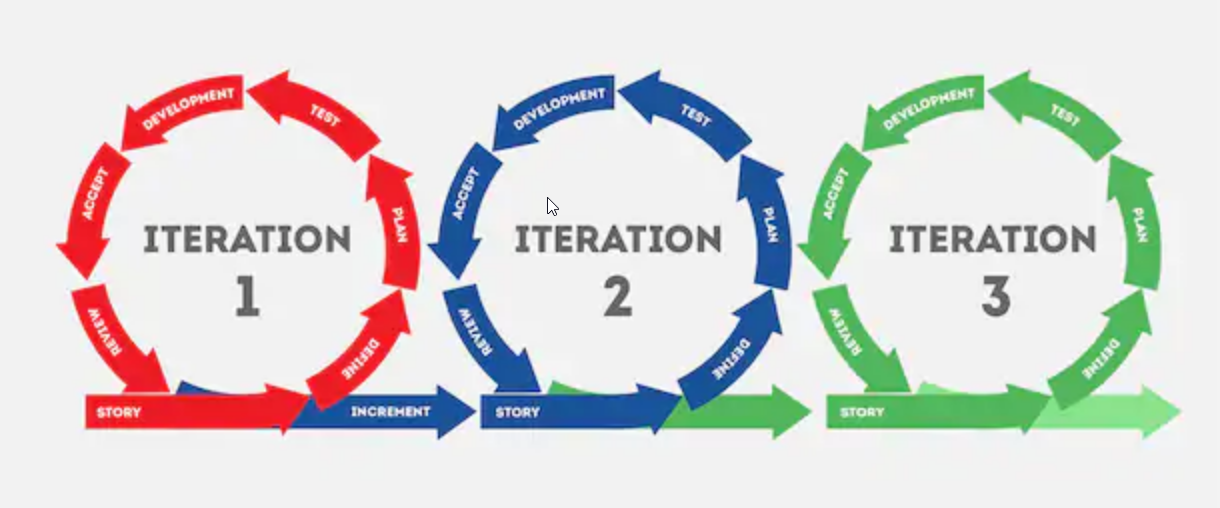
\includegraphics[scale=0.40]{assets/iteration.png}
      \caption{Iterative process project life cycle}
      \label{fig:iterationlifecycle}
\end{figure}
\paragraph*{Iterative}
The iterative aspect of a process enables the repetition of tasks. As a result, the deliverables are produced gradually. For example, when a use case is iterated, additional material is added to the description of the use case—such as alternative flows within the use case. The iterative approach encourages a slow and steady philosophy rather than hurrying and finishing up a deliverable in the first attempt.
Deliverables are gradually matured by undertaking at least three iterations across multiple other deliverables. For example, while following an iterative process one might move from an initial use case to another use case in another diagram, then identify classes and draw a sequence diagram before coming back to the original use case and completing it.
\paragraph*{Incremental}
The incremental aspect of a process enables adding new elements and diagrams to an existing deliverable. An example is to add new packages to existing or developing packages. New requirements are thus discovered and modeled incrementally. This incremental aspect of the process enables the creation of parts of a system in as complete a manner as possible before proceeding with the development of additional parts of the system. The incremental aspect of a process often goes hand in hand with the iterative aspect. For example, while a new deliverable is incrementally added (a new use case), an existing deliverable is iteratively augmented during a later iteration (e.g., additional steps added to a use case).
\clearpage
\subsection{Monitoring and planning}
\subsubsection*{Monitoring}
Breaking down a project into subparts to enable controlled execution and monitoring of the project.\\
Figure \ref{fig:bos} shows how the business objective is divided into subparts. to arrive at acceptable performance criteria of the system, the BO gets further divided into smaller parts or subject areas.
\begin{figure}[!ht]
      \center
      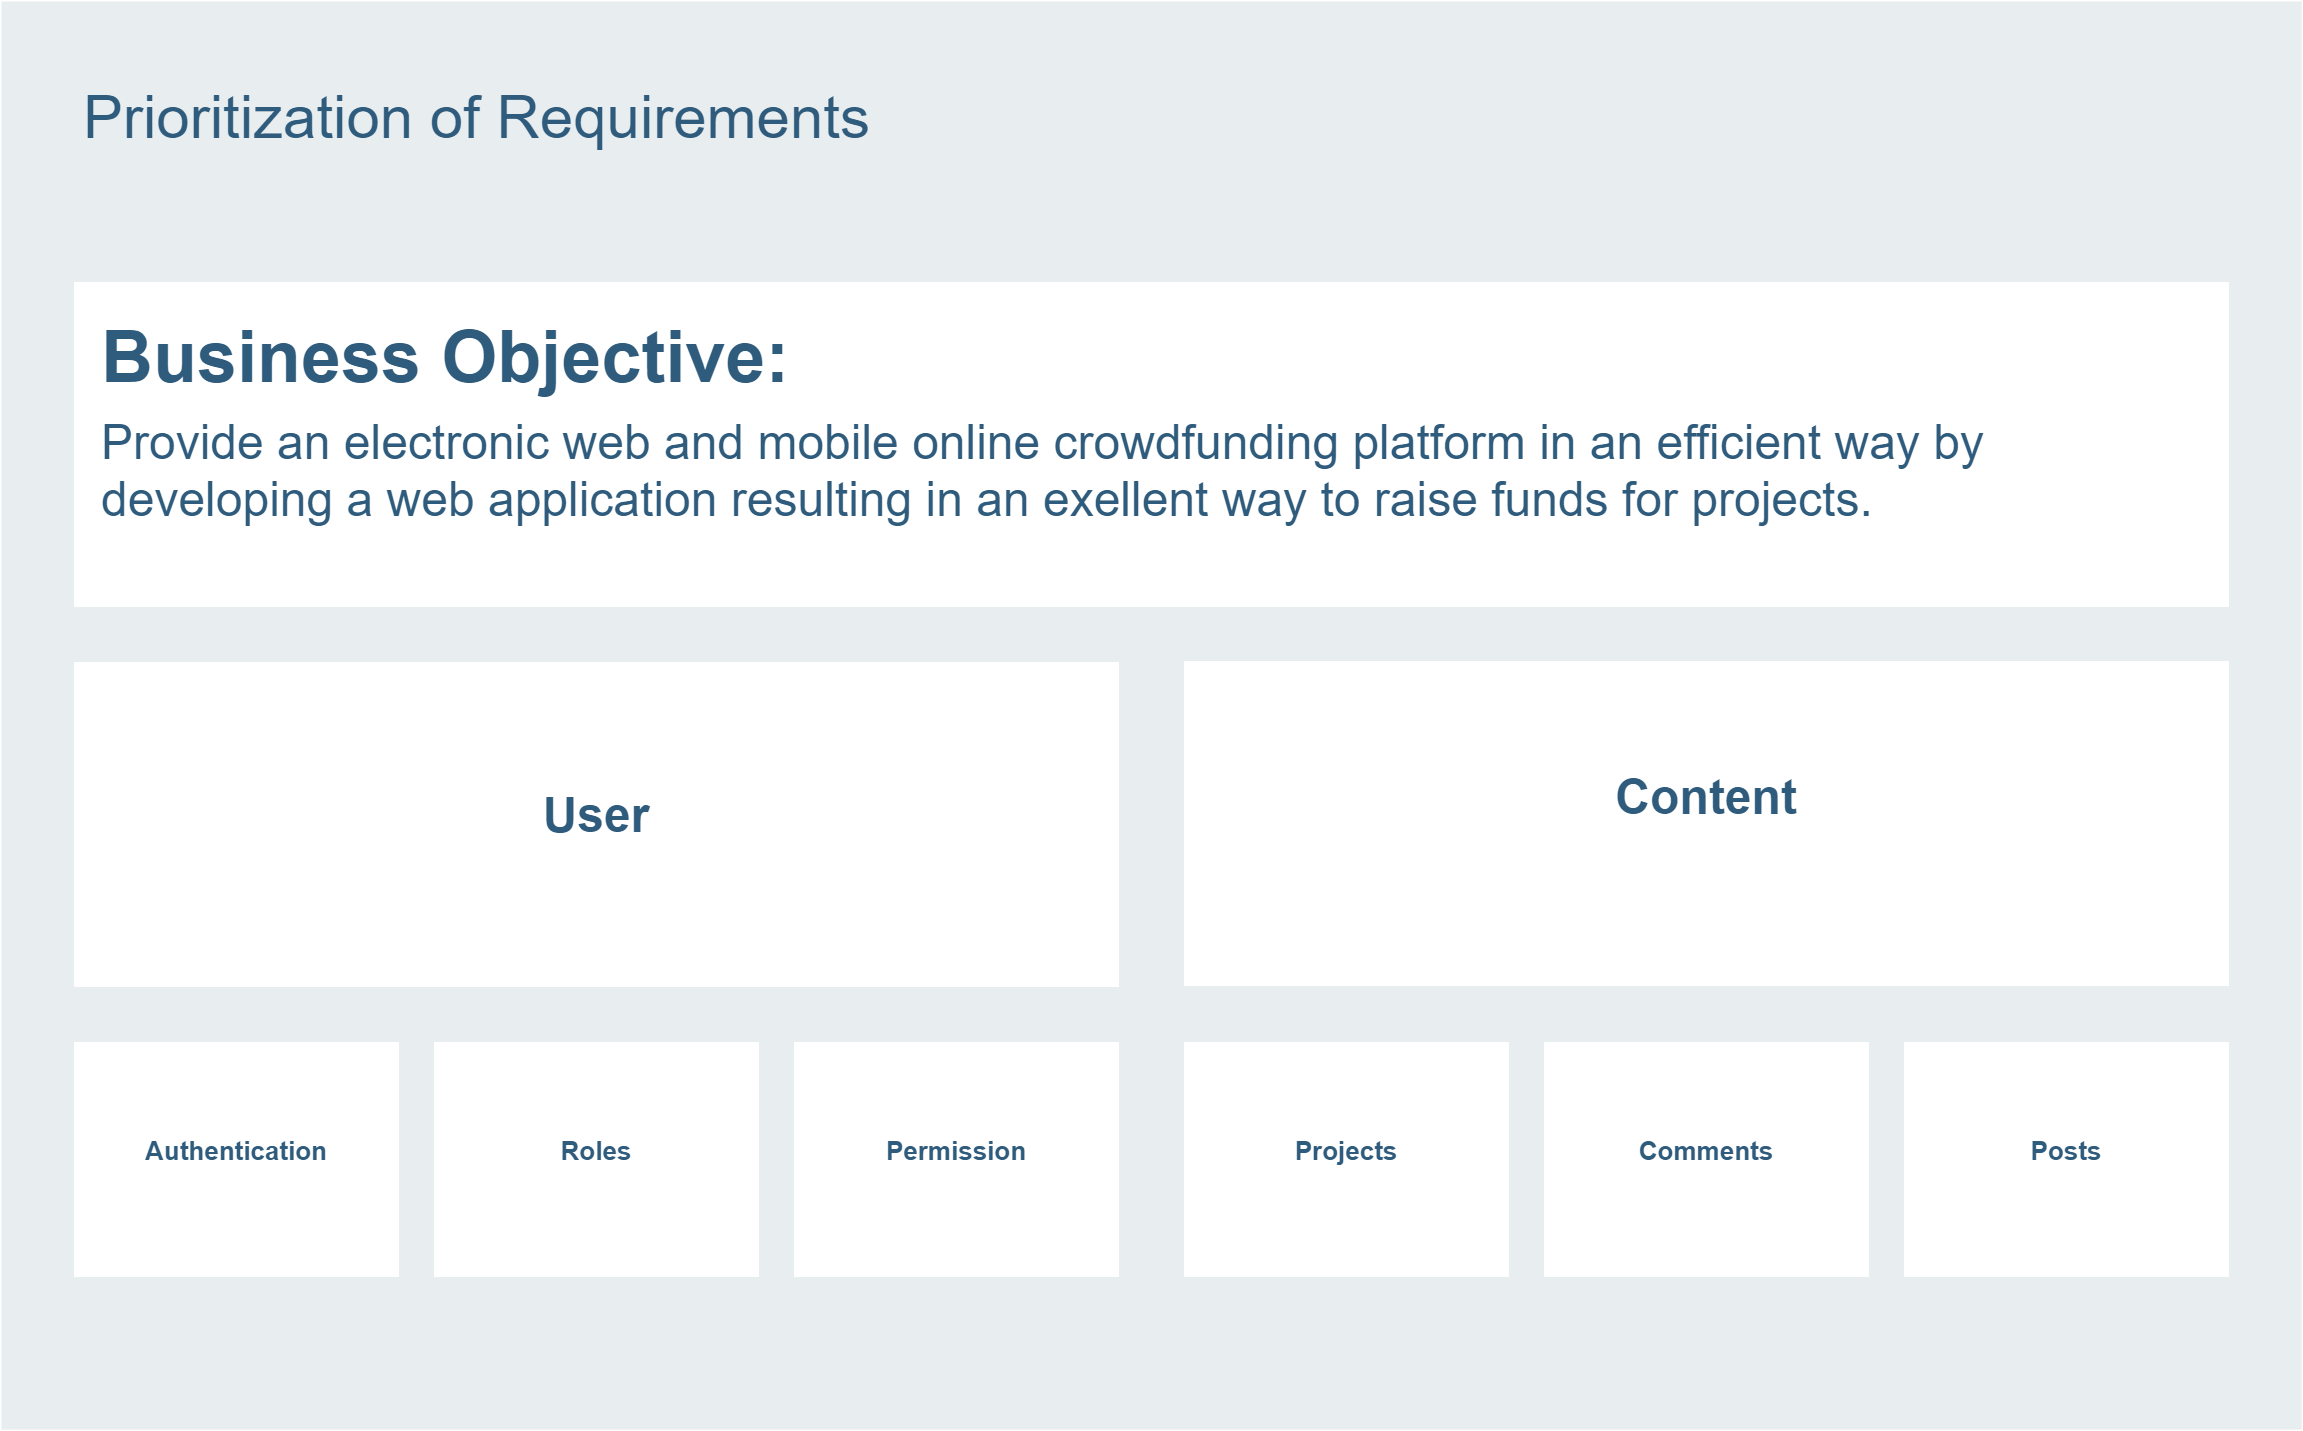
\includegraphics[scale=0.20]{assets/bos.png}
      \caption{Iterative process project life cycle}
      \label{fig:bos}
\end{figure}
\subsubsection*{Planning}
Provide precise routing of one or more business processes with opportunities to optimize on time and costs associated with the processes.
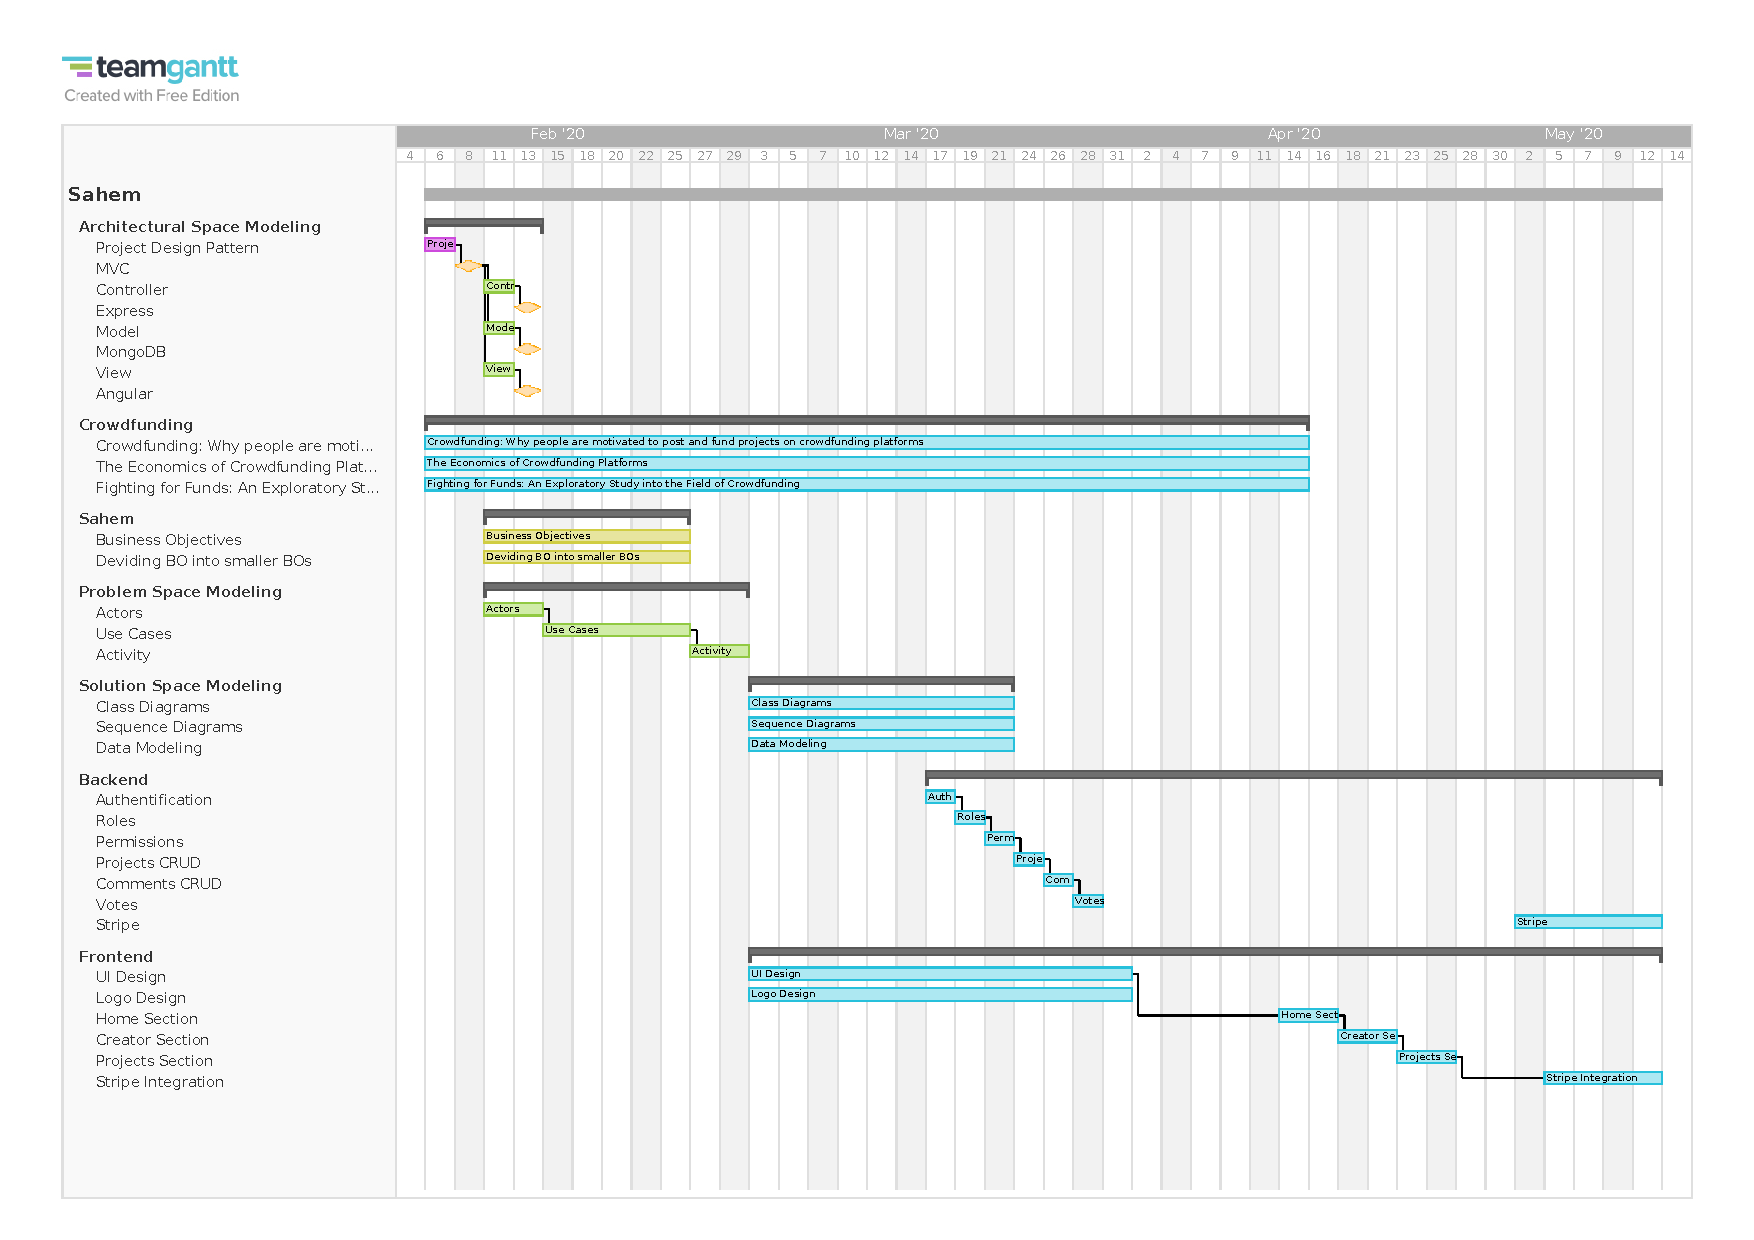
\includepdf[pages=-,angle=90,]{assets/ganttchart.pdf}

    \cleardoublepage%

    % @Author: Taha Bouhsine


%%%%%%%%%%%%%%%%%%%%%%%%%%%%
% CHAPTER                  %
%%%%%%%%%%%%%%%%%%%%%%%%%%%%
\setcounter{mtc}{8}
\chapter{Analysis And Design}%
\label{chap:chapter_two}
\minitoc
%%%%%%%%%%%%%%%%%%%%%%%%%%%%
% SECTION                  %
%%%%%%%%%%%%%%%%%%%%%%%%%%%%
\section{General description of the platform}

% \begin{description}\addtolength{\itemsep}{-0.35\baselineskip}%
%   \item[\textbullet~\bfseries Menu Item] \hfill \\%
%         Menu Description.~\\%
%         {\textbf{Focus topics:~}\emph{Topic one, topic two, topic three, ...}}%
%         %
%   \item[\textbullet~\bfseries Menu Item] \hfill \\%
%         Menu Description.~\\%
%         {\textbf{Focus topics:~}\emph{Topic one, topic two, topic three, ...}}%
%         %
%   \item[\textbullet~\bfseries Menu Item] \hfill \\%
%         Menu Description.~\\%
%         {\textbf{Focus topics:~}\emph{Topic one, topic two, topic three, ...}}%
% \end{description}

% Also bullets such as:%
% \begin{itemize}\addtolength{\itemsep}{-0.35\baselineskip}%
%   \item One%
%   \item Two%
%   \item Three%
%   \item Four%
%   \item \ldots%
% \end{itemize}%
% %

\section{Specification of requirements}
We will proceed according to the UML method which consists of identifying and modeling the various business processes in order to easily migrate to an object architecture from a static and dynamic point of view. This analysis presents a total abstraction being independent of any technology or implementation.


The specification of the needs will allow us to have a better approach of the users, the functionalities and the relationship between the two. It will be in the form of a use case. For this we will proceed as follows:

Identification of requirements.
Identification of the actors of the system.
Identification of use cases.
Description of use cases.
Grouping of use cases into packages.


\subsection{requirements}
The requirements that the client has put on the end-product were divided into basic functionalities and optional functionalities

The Client’s basic functionalities are:
\begin{enumerate}
    \item
          Account management: create an account, login, profile, settings, personal info,
          personal dashboard.
    \item
          Start a campaign: send in a proposal for a campaign (webform).
    \item
          Share function: functionality so that a campaign can be shared within social networks, such as Facebook, Instagram, LinkedIn, Twitter, and potentially Pinterest and Google.
    \item
          Contribution invitation: functionality to send out concrete requests to contribute a certain amount
          within the personal social network.
    \item
          Payment function: contributor should be able to pay their ticket through Credit Card.
    \item
          Review function: contributors should have the opportunity to give reviews about and react to events
          that have taken place.
    \item
          Countdown timer: a timer that shows how much time a campaign has left until it closes.
    \item
          Current overview: each campaign should show for example the amount of tickets sold/amount of investors, the amount of money raised so far and the goal amount to be raised.
\end{enumerate}


The Client’s optional functionalities are:

\begin{enumerate}
    \item
          Personalized recommendations (recommender system): the system will advice, suggest or give concrete offers. Logged-in visitors see a personalized recommendation based on social profiles and the
          platform’s web page content and actions.
    \item
          Share option via Whatsapp
    \item
          Online helpdesk: chat possibility with a helpdesk worker.
    \item
          Communication tools: communication possibilities with other members and/or the organization of an
          event via chat.
    \item
          Connection with social media: e.g. Facebook application for special opportunities and/or campaigns
          that enabled even more interaction with the target group.
    \item
          Social login: login with a social account.
    \item
          Wallet: deposit money in your personal wallet, which enables you to make several contributions by
          paying with the money in your wallet.
    \item
          Recruit function: a tool to gather more contributors. A contributor can share a campaign within their
          own personal social networks.
    \item
          Notifications: reminders and/or messages related to upcoming events and updates of events.
    \item
          Mobile App: extra functionalities through the use of a camera and GPS on the actual event: e.g. picture/video upload to the website or live visitor numbers.

    \item
          Agenda/calender: an overview that shows which events will take place on which dates (including events
          that have already taken place).
    \item
          Newsletter: send an overview of the events to members of the platform community or to a certain
          selection.
    \item
          Promotion function: functionality to share and promote events on different levels: community (everyone), events (only participants of a specific event), social media (within social networks).
    \item
          Campaign management: management tools for the event organization.
    \item
          Reports/statistics: data analyses, tools for advanced analysis of the web page visits.
\end{enumerate}




\subsection{Identification of actors}
In UML we don't use the term users but actors. A player in a system is an entity external to this system that interacts (data entry, reception of information, etc.) with it. The actors make it possible to define the interface that the system will offer to its environment.And also the actor groups together several users who have the same role. And to find actors it will be necessary to identify the different roles that will have to play its users.
In order to facilitate identification, we can imagine this: everything that is outside and interacts with the system is an actor, everything that is inside is a functionality to be realized.
The different actors of the studied system are:

\begin{enumerate}
    \item  Creator.
    \item  Funder.
    \item  Administrator.
    \item  Visitor.

\end{enumerate}

\subsection{Identification of objectives and use cases}
A use case described in the form of actions and reactions, the behavior of a system from a user point of view. It must add value to the actor concerned. Each use case contains a list of functionalities which will be detailed in the following section.

We will first determine the objectives that will allow us to deduce the use cases and all this:
\begin{longtable}{|m{10em}|m{10em}|m{10em}|}\hline
    \multirow{4}{*}{Administration management} & \multirow{2}{*}{Authentication}       & Authentication                          \\\cline{3-3}
                                               &                                       & Registration                            \\\cline{2-3}
                                               & \multirow{5}{*}{User Maintainance}    & Add User                                \\\cline{3-3}
                                               &                                       & Modify User                             \\\cline{3-3}
                                               &                                       & Delete User                             \\\cline{3-3}
                                               &                                       & Consult the information of a user       \\\cline{3-3}
                                               &                                       & Show the list of users                  \\\cline{2-3}
                                               & \multirow{2}{*}{Roles}                & Show users by roles                     \\\cline{3-3}
                                               &                                       & Modify a user's role                    \\\cline{2-3}
                                               & \multirow{1}{*}{Statistics}           & Access the statistics of the plateforme \\\hline
    \multirow{4}{*}{Fundraiser's managment}    & \multirow{3}{*}{Creator's Monitoring} & Personal information modification       \\\cline{3-3}
                                               &                                       & Access a creator profile                \\\cline{3-3}
                                               &                                       & Desactivate an Account                  \\\cline{2-3}
                                               & \multirow{2}{*}{Funds Monitoring}     & Fund a project                          \\\cline{3-3}
                                               &                                       & Confirm funding a project               \\\cline{3-3}
                                               &                                       & List of previous funds                  \\\cline{2-3}
                                               & \multirow{6}{*}{Projects Monitoring}  & Create a project                        \\\cline{3-3}
                                               &                                       & Edit a project                          \\\cline{3-3}
                                               &                                       & Delete a project                        \\\cline{3-3}
                                               &                                       & Like a project                          \\\cline{3-3}
                                               &                                       & Share a project                         \\\cline{3-3}
                                               &                                       & Comment on a project                    \\\cline{2-3}
                                               & \multirow{2}{*}{Search}               & Search a project by name                \\\cline{3-3}
                                               &                                       & Show Fundraisers by category            \\\hline
    \multirow{2}{*}{Payment management}        & \multirow{1}{*}{Billing}              & Show the bill                           \\\cline{2-3}
                                               & \multirow{1}{*}{Online Payment}       & Choose payment method                   \\\hline

    \caption{Identification of objectives and use cases}
    \label{tab:id_objec_uc}
\end{longtable}

%%%%%%%%%%%%%%%%%%%%%%%%%%%%
% SECTION                  %
%%%%%%%%%%%%%%%%%%%%%%%%%%%%
\section{Analyse fonctionnelle}
usecase
%%%%%%%%%%%%%%%%%%%%%%%%%%%%
% SECTION                  %
%%%%%%%%%%%%%%%%%%%%%%%%%%%%
\section{Analyse dynamique}
activity  squence
%%%%%%%%%%%%%%%%%%%%%%%%%%%%
% SECTION                  %
%%%%%%%%%%%%%%%%%%%%%%%%%%%%
\section{Analyse structurelle}
class
    \cleardoublepage%

    % @Author: Taha Bouhsine


%%%%%%%%%%%%%%%%%%%%%%%%%%%%
% CHAPTER                  %
%%%%%%%%%%%%%%%%%%%%%%%%%%%%
\chapter{Tools, Technologies and Languages Used}%
\label{chap:chapter_two}
\section{Mean Stack}
\begin{figure}[!ht]
    \center
    
\includegraphics[scale=0.30]{assets/meanstack.png}
\end{figure}

While the name sounds like “mean”, it actually stands for the software pieces that are used to create a particular development stack: MongoDB, ExpressJS, Angular, and NodeJS. One of the biggest advantages of using this particular development stack is the ability to allow developers to use one consistent data model across the stack, using JSON and BSON (for MongoDB). This allows for quick transitions between the various pieces of the stack, especially when a single programmer has to handle more than one portion of the stack.

\begin{figure}[!ht]
    \center
    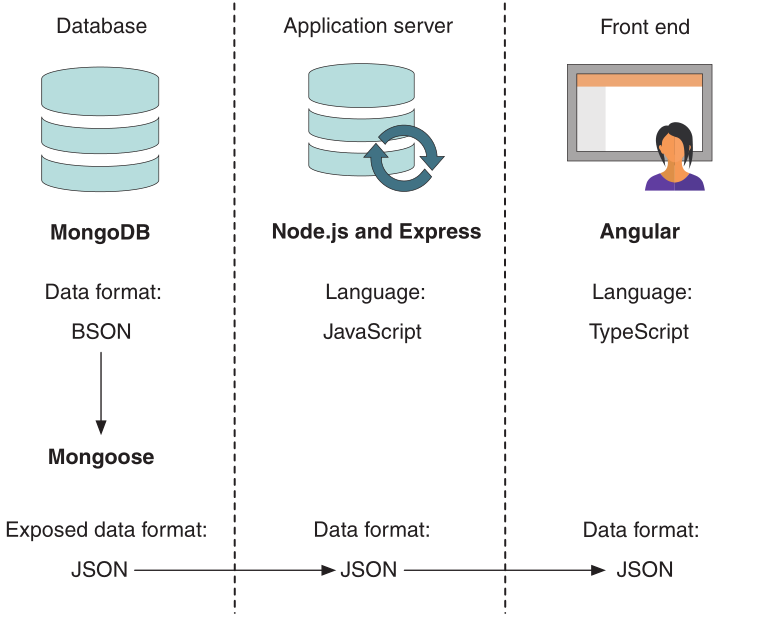
\includegraphics[scale=0.60]{assets/mean.png}
    \caption{Mean Stack}
    \label{fig:mean}
\end{figure}

\section{Model View Controller Design Pattern}

The Model View Controller (MVC) design pattern specifies that an application consist of a data model, presentation information, and control information. The pattern requires that each of these be separated into different objects.

MVC is more of an architectural pattern, but not for complete application. MVC mostly relates to the UI / interaction layer of an application. We’re still going to need business logic layer, maybe some service layer and data access layer.



\begin{enumerate}
    \item Model contains only the pure application data, it contains no logic describing how to present the data to a user.
    \item View presents the model’s data to the user. The view knows how to access the model’s data, but it does not know what this data means or what the user can do to manipulate it.
    \item Controller exists between the view and the model. It listens to events triggered by the view (or another external source) and executes the appropriate reaction to these events. In most cases, the reaction is to call a method on the model. Since the view and the model are connected through a notification mechanism, the result of this action is then automatically reflected in the view.
\end{enumerate}

\begin{figure}[!ht]
    \center
    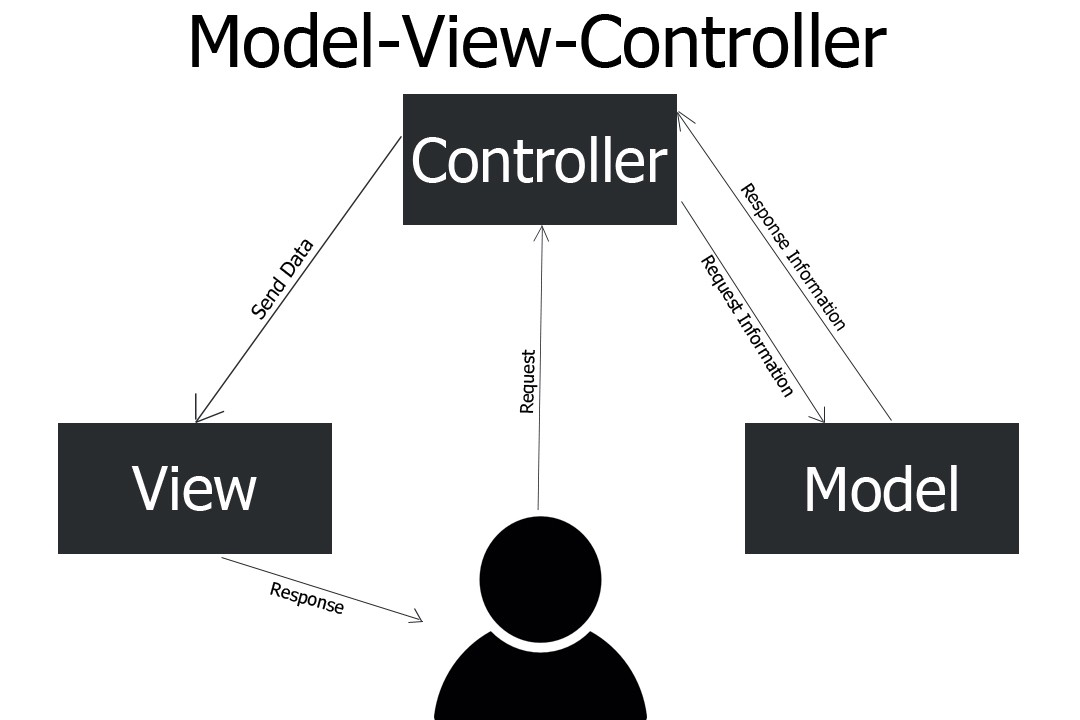
\includegraphics[scale=0.30]{assets/mvc.jpg}
    \caption{Model View Controller}
    \label{fig:mvc}
\end{figure}

\section{Representational State Transfer Architecture}
REST, or REpresentational State Transfer, is an architectural style for providing standards between computer systems on the web, making it easier for systems to communicate with each other. REST-compliant systems, often called RESTful systems, are characterized by how they are stateless and separate the concerns of client and server. We will go into what these terms mean and why they are beneficial characteristics for services on the Web.




\section{Software as a Service}
Software as a Service or SaaS , which allows us to set up services, such as application servers and databases, as needed to create the apps we need. This type of system typically works in a cloud or hybrid cloud environment, which often makes provisioning of servers and software as simple as entering some configurations and clicking a button.

This type of setup is perfect for the MEAN stack, as each piece of the MEAN stack is easily placed into the cloud and thus can be easily provisioned, so they are widely available on SaaS services and can be used quickly when needed. If we are looking for a good development stack, the MEAN stack has much to offer for IT management as well as for developers!



\section{Monolithic Applications}

If all the functionalities of a project exists in a single codebase, then that application is known as monolithic application. We all must have designed a monolithic application in our lives in which we were given a problem statement and were asked to design a system with various functionalities. We design our application in various layers like presentation, service and persistence and then deploy that codebase as single jar/war file. This is nothing but a monolithic application where “mono” represents the single codebase containing all the required functionalities.
\begin{figure}[!ht]
    \center
    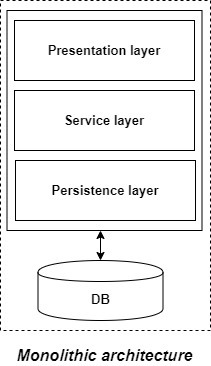
\includegraphics[scale=0.60]{assets/monolithic.jpg}
    \caption{Monolithic Applications}
    \label{fig:monoapp}
\end{figure}

Disadvantages of Monolithic applications:
\begin{enumerate}
    \item
          It becomes too large in size with time and hence, difficult to manage.
    \item
          We need to redeploy the whole application even for a small change.
    \item
          As the size of the application increases, its start-up and deployment time also increases.
    \item
          For any new developer joining the project, it is very difficult to understand the logic of large Monolithic application even if his responsibility is related to a single functionality.
    \item
          Even if a single part of the application is facing a large load/traffic, we need to deploy the instances of the whole application in multiple servers. It is very inefficient and takes up more resources unnecessarily. Hence, horizontal scaling is not feasible in monolithic applications.
    \item
          It is very difficult to adopt any new technology which is well suited for a particular functionality as it affects the whole application, both in terms of time and cost.
    \item
          It is not very reliable as a single bug in any module can bring down the whole monolithic application.
\end{enumerate}
Advantages of monolithic applications:
\begin{enumerate}
    \item
          Simple to develop relative to microservices where skilled developers are required in order to identify and develop the services.
    \item
          Easier to deploy as only a single jar/war file is deployed.
    \item
          Relatively easier and simple to develop in comparison to microservices architecture.
    \item
          The problems of network latency and security are relatively less in comparison to microservices architecture.
\end{enumerate}


\section{Conception}
\subsection{Unified Modeling Language}
\subsection{PlantUml}
PlantUML is an open-source tool allowing users to create UML diagrams from a plain text language. The language of PlantUML is an example of a Domain-specific language. It uses Graphviz software to lay out its diagrams. It has been used to allow blind students to work with UML. PlantUML also helps blind software engineers to design and read UML diagrams.


\subsection{Gantt chart}
A gantt chart is a horizontal bar chart that visually represents a project plan over time. Modern gantt charts typically show us the status of—as well as who’s responsible for—each task in the project.

In other words, a gantt chart is a super-simple way to keep us out of a project pinch!

What are the key parts of a gantt chart?
A gantt chart is made up of several different elements:
\begin{enumerate}
    \item
          Task list: Runs vertically down the left of the gantt chart to describe project work and may be organized into groups and subgroups
    \item
          Timeline: Runs horizontally across the top of the gantt chart and shows months, weeks, days, and years
    \item
          Dateline: A vertical line that highlights the current date on the gantt chart
    \item
          Bars: Horizontal markers on the right side of the gantt chart that represent tasks and show progress, duration, and start and end dates
    \item
          Milestones: Yellow diamonds that call out major events, dates, decisions, and deliverables
    \item
          Dependencies: Light gray lines that connect tasks that need to happen in a certain order
    \item
          Progress: Shows how far along work is and may be indicated by \% Complete and/or bar shading
    \item
          Resource assigned: Indicates the person or team responsible for completing a task
\end{enumerate}


\section{Design}
\subsection{Adobe Photoshop}
Adobe Photoshop is a software application for image editing and photo retouching for use on Windows or MacOS computers. Photoshop offers users the ability to create, enhance, or otherwise edit images, artwork, and illustrations. Changing backgrounds, simulating a real-life painting, or creating an alternative view of the universe are all possible with Adobe Photoshop. It is the most widely used software tool for photo editing, image manipulation, and retouching for numerous image and video file formats. The tools within Photoshop make it possible to edit both individual images as well as large batches of photos.
We used it to prototype and create our platform logo.
\subsection{Adobe XD}
Adobe XD is a vector-based user experience design tool for web apps and mobile apps, developed and published by Adobe Inc. It is available for macOS and Windows, although there are versions for iOS and Android to help preview the result of work directly on mobile devices. XD.


\section{Front-End}
We decided to go with the single page application instead of the multiple pages application and we will be using the following tools for the front end.
\subsection{HTML}
Hypertext Markup Language (HTML) is the standard markup language for documents designed to be displayed in a web browser. It can be assisted by technologies such as Cascading Style Sheets (CSS) and scripting languages such as JavaScript.

Web browsers receive HTML documents from a web server or from local storage and render the documents into multimedia web pages. HTML describes the structure of a web page semantically and originally included cues for the appearance of the document.



\subsection{CSS}
Cascading Style Sheets (CSS) is a style sheet language used for describing the presentation of a document written in a markup language like HTML.[1] CSS is a cornerstone technology of the World Wide Web, alongside HTML and JavaScript.[2]

CSS is designed to enable the separation of presentation and content, including layout, colors, and fonts.[3] This separation can improve content accessibility, provide more flexibility and control in the specification of presentation characteristics, enable multiple web pages to share formatting by specifying the relevant CSS in a separate .css file, and reduce complexity and repetition in the structural content.


\subsection{Typescript}
TypeScript is an open-source programming language developed and maintained by Microsoft. It is a strict syntactical superset of JavaScript and adds optional static typing to the language. TypeScript is designed for development of large applications and transcompiles to JavaScript.[5] As TypeScript is a superset of JavaScript, existing JavaScript programs are also valid TypeScript programs.

TypeScript may be used to develop JavaScript applications for both client-side and server-side execution (as with Node.js or Deno). There are multiple options available for transcompilation. Either the default TypeScript Checker can be used,[6] or the Babel compiler can be invoked to convert TypeScript to JavaScript.

TypeScript supports definition files that can contain type information of existing JavaScript libraries, much like C++ header files can describe the structure of existing object files. This enables other programs to use the values defined in the files as if they were statically typed TypeScript entities. There are third-party header files for popular libraries such as jQuery, MongoDB, and D3.js. TypeScript headers for the Node.js basic modules are also available, allowing development of Node.js programs within TypeScript.

The TypeScript compiler is itself written in TypeScript and compiled to JavaScript. It is licensed under the Apache License 2.0. TypeScript is included as a first-class programming language in Microsoft Visual Studio 2013 Update 2 and later, beside C\# and other Microsoft languages. An official extension allows Visual Studio 2012 to support TypeScript as well. Anders Hejlsberg, lead architect of C\# and creator of Delphi and Turbo Pascal, has worked on the development of TypeScript.



\subsection{Angular 9}
Angular is an app-design framework and development platform for creating efficient and sophisticated single-page apps in html, css, and Typescript which is a superset of JavaScript. Angular provides built-in features for animation, http service, and materials which in turn have features such as auto-complete, navigation, toolbar, menus, etc. The code is written in Typescript, which compiles to JavaScript and displays the same in the browser.
\subsection{Hypertext Transfer Protocol}
The Hypertext Transfer Protocol (HTTP) is an application protocol for distributed, collaborative, hypermedia information systems. HTTP is the foundation of data communication for the World Wide Web, where hypertext documents include hyperlinks to other resources that the user can easily access, for example by a mouse click or by tapping the screen in a web browser.
\subsection{JSON}
JavaScript Object Notation (JSON) is an open standard file format, and data interchange format, that uses human-readable text to store and transmit data objects consisting of attribute–value pairs and array data types (or any other serializable value). It is a very common data format, with a diverse range of applications, such as serving as a replacement for XML in AJAX systems.

JSON is a language-independent data format. It was derived from JavaScript, but many modern programming languages include code to generate and parse JSON-format data. The official Internet media type for JSON is application/json. JSON filenames use the extension .json.



\section{Back-End}
\subsection{Javascript}
JavaScript often abbreviated as JS, is a programming language that conforms to the ECMAScript specification.[7] JavaScript is high-level, often just-in-time compiled, and multi-paradigm. It has curly-bracket syntax, dynamic typing, prototype-based object-orientation, and first-class functions.


\subsection{Node Js}
Node.js is an open source, cross-platform runtime environment for developing server-side and networking applications. Node.js applications are written in JavaScript, and can be run within the Node.js runtime on OS X, Microsoft Windows, and Linux.
Node.js also provides a rich library of various JavaScript modules which simplifies the development of web applications using Node.js to a great extent.

Following are some of the important features that make Node.js the first choice of software architects.
\begin{enumerate}
    \item
          Asynchronous and Event Driven: All APIs of Node.js library are asynchronous, that is, non-blocking. It essentially means a Node.js based server never waits for an API to return data. The server moves to the next API after calling it and a notification mechanism of Events of Node.js helps the server to get a response from the previous API call.
    \item
          Very Fast: Being built on Google Chrome's V8 JavaScript Engine, Node.js library is very fast in code execution.
    \item
          Single Threaded but Highly Scalable: Node.js uses a single threaded model with event looping. Event mechanism helps the server to respond in a non-blocking way and makes the server highly scalable as opposed to traditional servers which create limited threads to handle requests. Node.js uses a single threaded program and the same program can provide service to a much larger number of requests than traditional servers like Apache HTTP Server.
    \item
          No Buffering: Node.js applications never buffer any data. These applications simply output the data in chunks.
    \item
          License: Node.js is released under the MIT license
\end{enumerate}





\subsection{Express Js}
ExpressJS is a web application framework that provides us with a simple API to build websites, web apps and back ends. With ExpressJS, we need not worry about low level protocols, processes, etc.
Express provides a minimal interface to build our applications. It provides us the tools that are required to build our app. It is flexible as there are numerous modules available on npm, which can be directly plugged into Express.
Express was developed by TJ Holowaychuk and is maintained by the Node.js foundation and numerous open source contributors.



\subsection{MongoDB}
MongoDB is a cross-platform, document oriented database that provides, high performance, high availability, and easy scalability. MongoDB works on concept of collection and document.
\begin{enumerate}
    \item
          Database\\
          Database is a physical container for collections. Each database gets its own set of files on the file system. A single MongoDB server typically has multiple databases.
    \item
          Collection\\
          Collection is a group of MongoDB documents. It is the equivalent of an RDBMS table. A collection exists within a single database. Collections do not enforce a schema. Documents within a collection can have different fields. Typically, all documents in a collection are of similar or related purpose.
    \item
          Document\\
          A document is a set of key-value pairs. Documents have dynamic schema. Dynamic schema means that documents in the same collection do not need to have the same set of fields or structure, and common fields in a collection's documents may hold different types of data.
\end{enumerate}





\subsection{Mongoose}
Mongoose is an Object Data Modeling (ODM) library for MongoDB and Node.js. It manages relationships between data, provides schema validation, and is used to translate between objects in code and the representation of those objects in MongoDB.


\section{Development}
\subsection{Visual Studio Code}
DescriptionVisual Studio Code is a source-code editor developed by Microsoft for Windows, Linux and macOS. It includes support for debugging, embedded Git control and GitHub, syntax highlighting, intelligent code completion, snippets, and code refactoring.


\subsection{MongoDB Compass Community}
MongoDB Compass is the defacto GUI tool for MongoDB much like MySQL Workbench is MySQL’s associated tool. It allows us to visually explore our data, run ad hoc queries, interact with our data with full CRUD functionality, as well as view and optimize our queries’ performance.



\subsection{Postman}
Postman is an interactive and automatic tool for verifying the APIs of our project. Postman is a Google Chrome app for interacting with HTTP APIs. It presents us with a friendly GUI for constructing requests and reading responses. It works on the backend, and makes sure that each API is working as intended.

In Postman, we create a request, and Postman looks at the response to make sure it has the element we want in it. As it is an automation tool, it drastically improves testing time and quality of the project. It helps in the early detection of bugs that might sprout at later stages and cause more damage to the system.

Postman is the way to streamline the process of API testing. All APIs that we create and deploy first rigorously go through Postman so that any major or show stopper bugs are identified on time and fewer bugs leak through to later stages.



\subsection{Git}
% Git is a version control system for tracking changes in computer files and coordinating work on those files among multiple people. It is primarily used for source code management in software development, but it can be used to keep track of changes in any set of files. As a distributed revision control system it is aimed at speed, data integrity, and support for distributed, non-linear workflows.
Git is a distributed revision control and source code management system that
allows several people to work on the same codebase at the same time on different
computers and networks. These can be pushed together, with all changes stored and
recorded. It’s also possible to roll back to an earlier state if necessary.
\subsection{Github}
At a high level, GitHub is a website and cloud-based service that helps developers store and manage their code, as well as track and control changes to their code. To understand exactly what GitHub is, we need to know two connected principles:
\begin{enumerate}
    \item Version control
    \item Git
\end{enumerate}

\subsection{Github Desktop}
GitHub Desktop is a fast and easy way to contribute to projects from Windows and OS X, whether we are a seasoned users or new users, GitHub Desktop is designed to simplify all processes and workflow in our GitHub. GitHub Desktop is an open-source Electron-based GitHub app. It is written in TypeScript and uses React.


\subsection{Boost Note}
% Boostnote is an Open source note-taking app for programmers.
% Boostnote is niche tool because designed for programmers, but we are passionate for it.
% It focuses on writing Markdown note and code snippet quickly, can organized in a better way.
% You can sync data to multi-devices(Mac, Windows, Linux, Android and iOS) via Dropbox.
% Boostnote is not an app suitable for everyone, it ‘s a handy note-taking app for programmers.
% Boostnote has two main features.
% Markdown note
% Since Boostnote is a Markdown editor, mainly write with markdown.
% Content is automatically saved while editing notes.
% Since preview could be viewed with one touch, you can immediately check the Markdown preview you are writing.
% Snippet note
% In the code snippet, you can highlight code syntax in over 100 languages ​​such as Javascript, Python, HTML, etc., and save multiple code snippets in one note.
% The indent and tab size can be set from the editor window.


\subsection{Latex}
\latex{} is a tool used to create professional-looking documents. It is based on the WYSIWYM (what we see is what we mean) idea, meaning we only have focus on the contents of our document and the computer will take care of the formatting. Instead of spacing out text on a page to control formatting, as with Microsoft Word or LibreOffice Writer, users can enter plain text and let LATEX take care of the rest.
\subsection{MiKTex}
% MiKTeX provides the tools necessary to prepare documents using the TeX/LaTeX markup language, as well as a simple tex editor: TeXworks.

\subsection{Tex Live}
% TeX Live is intended to be a straightforward way to get up and running with the TeX document production system. It provides a comprehensive TeX system with binaries for most flavors of Unix, including GNU/Linux, macOS, and also Windows. It includes all the major TeX-related programs, macro packages, and fonts that are free software, including support for many languages around the world. Many operating systems provide it via their own distributions.



\subsection{Markdown}
Markdown is a lightweight markup language with plain-text-formatting syntax. Its design allows it to be converted to many output formats, but the original tool by the same name only supports HTML. Markdown is often used to format readme files, for writing messages in online discussion forums, and to create rich text using a plain text editor.
\subsection{Marp}
Marp is the ecosystem to write our presentation with plain Markdown
\section{Deployment}
\subsection{Google Cloud Platform}
\subsection{MongoDB Atlas}


    \cleardoublepage%

    

    % % @Author: Taha Bouhsine


%%%%%%%%%%%%%%%%%%%%%%%%%%%%
% CHAPTER                  %
%%%%%%%%%%%%%%%%%%%%%%%%%%%%
\setcounter{mtc}{8}
\chapter{Analysis And Design}%
\label{chap:chapter_two}
\minitoc
%%%%%%%%%%%%%%%%%%%%%%%%%%%%
% SECTION                  %
%%%%%%%%%%%%%%%%%%%%%%%%%%%%
\section{General description of the platform}

% \begin{description}\addtolength{\itemsep}{-0.35\baselineskip}%
%   \item[\textbullet~\bfseries Menu Item] \hfill \\%
%         Menu Description.~\\%
%         {\textbf{Focus topics:~}\emph{Topic one, topic two, topic three, ...}}%
%         %
%   \item[\textbullet~\bfseries Menu Item] \hfill \\%
%         Menu Description.~\\%
%         {\textbf{Focus topics:~}\emph{Topic one, topic two, topic three, ...}}%
%         %
%   \item[\textbullet~\bfseries Menu Item] \hfill \\%
%         Menu Description.~\\%
%         {\textbf{Focus topics:~}\emph{Topic one, topic two, topic three, ...}}%
% \end{description}

% Also bullets such as:%
% \begin{itemize}\addtolength{\itemsep}{-0.35\baselineskip}%
%   \item One%
%   \item Two%
%   \item Three%
%   \item Four%
%   \item \ldots%
% \end{itemize}%
% %

\section{Specification of requirements}
We will proceed according to the UML method which consists of identifying and modeling the various business processes in order to easily migrate to an object architecture from a static and dynamic point of view. This analysis presents a total abstraction being independent of any technology or implementation.


The specification of the needs will allow us to have a better approach of the users, the functionalities and the relationship between the two. It will be in the form of a use case. For this we will proceed as follows:

Identification of requirements.
Identification of the actors of the system.
Identification of use cases.
Description of use cases.
Grouping of use cases into packages.


\subsection{requirements}
The requirements that the client has put on the end-product were divided into basic functionalities and optional functionalities

The Client’s basic functionalities are:
\begin{enumerate}
    \item
          Account management: create an account, login, profile, settings, personal info,
          personal dashboard.
    \item
          Start a campaign: send in a proposal for a campaign (webform).
    \item
          Share function: functionality so that a campaign can be shared within social networks, such as Facebook, Instagram, LinkedIn, Twitter, and potentially Pinterest and Google.
    \item
          Contribution invitation: functionality to send out concrete requests to contribute a certain amount
          within the personal social network.
    \item
          Payment function: contributor should be able to pay their ticket through Credit Card.
    \item
          Review function: contributors should have the opportunity to give reviews about and react to events
          that have taken place.
    \item
          Countdown timer: a timer that shows how much time a campaign has left until it closes.
    \item
          Current overview: each campaign should show for example the amount of tickets sold/amount of investors, the amount of money raised so far and the goal amount to be raised.
\end{enumerate}


The Client’s optional functionalities are:

\begin{enumerate}
    \item
          Personalized recommendations (recommender system): the system will advice, suggest or give concrete offers. Logged-in visitors see a personalized recommendation based on social profiles and the
          platform’s web page content and actions.
    \item
          Share option via Whatsapp
    \item
          Online helpdesk: chat possibility with a helpdesk worker.
    \item
          Communication tools: communication possibilities with other members and/or the organization of an
          event via chat.
    \item
          Connection with social media: e.g. Facebook application for special opportunities and/or campaigns
          that enabled even more interaction with the target group.
    \item
          Social login: login with a social account.
    \item
          Wallet: deposit money in your personal wallet, which enables you to make several contributions by
          paying with the money in your wallet.
    \item
          Recruit function: a tool to gather more contributors. A contributor can share a campaign within their
          own personal social networks.
    \item
          Notifications: reminders and/or messages related to upcoming events and updates of events.
    \item
          Mobile App: extra functionalities through the use of a camera and GPS on the actual event: e.g. picture/video upload to the website or live visitor numbers.

    \item
          Agenda/calender: an overview that shows which events will take place on which dates (including events
          that have already taken place).
    \item
          Newsletter: send an overview of the events to members of the platform community or to a certain
          selection.
    \item
          Promotion function: functionality to share and promote events on different levels: community (everyone), events (only participants of a specific event), social media (within social networks).
    \item
          Campaign management: management tools for the event organization.
    \item
          Reports/statistics: data analyses, tools for advanced analysis of the web page visits.
\end{enumerate}




\subsection{Identification of actors}
In UML we don't use the term users but actors. A player in a system is an entity external to this system that interacts (data entry, reception of information, etc.) with it. The actors make it possible to define the interface that the system will offer to its environment.And also the actor groups together several users who have the same role. And to find actors it will be necessary to identify the different roles that will have to play its users.
In order to facilitate identification, we can imagine this: everything that is outside and interacts with the system is an actor, everything that is inside is a functionality to be realized.
The different actors of the studied system are:

\begin{enumerate}
    \item  Creator.
    \item  Funder.
    \item  Administrator.
    \item  Visitor.

\end{enumerate}

\subsection{Identification of objectives and use cases}
A use case described in the form of actions and reactions, the behavior of a system from a user point of view. It must add value to the actor concerned. Each use case contains a list of functionalities which will be detailed in the following section.

We will first determine the objectives that will allow us to deduce the use cases and all this:
\begin{longtable}{|m{10em}|m{10em}|m{10em}|}\hline
    \multirow{4}{*}{Administration management} & \multirow{2}{*}{Authentication}       & Authentication                          \\\cline{3-3}
                                               &                                       & Registration                            \\\cline{2-3}
                                               & \multirow{5}{*}{User Maintainance}    & Add User                                \\\cline{3-3}
                                               &                                       & Modify User                             \\\cline{3-3}
                                               &                                       & Delete User                             \\\cline{3-3}
                                               &                                       & Consult the information of a user       \\\cline{3-3}
                                               &                                       & Show the list of users                  \\\cline{2-3}
                                               & \multirow{2}{*}{Roles}                & Show users by roles                     \\\cline{3-3}
                                               &                                       & Modify a user's role                    \\\cline{2-3}
                                               & \multirow{1}{*}{Statistics}           & Access the statistics of the plateforme \\\hline
    \multirow{4}{*}{Fundraiser's managment}    & \multirow{3}{*}{Creator's Monitoring} & Personal information modification       \\\cline{3-3}
                                               &                                       & Access a creator profile                \\\cline{3-3}
                                               &                                       & Desactivate an Account                  \\\cline{2-3}
                                               & \multirow{2}{*}{Funds Monitoring}     & Fund a project                          \\\cline{3-3}
                                               &                                       & Confirm funding a project               \\\cline{3-3}
                                               &                                       & List of previous funds                  \\\cline{2-3}
                                               & \multirow{6}{*}{Projects Monitoring}  & Create a project                        \\\cline{3-3}
                                               &                                       & Edit a project                          \\\cline{3-3}
                                               &                                       & Delete a project                        \\\cline{3-3}
                                               &                                       & Like a project                          \\\cline{3-3}
                                               &                                       & Share a project                         \\\cline{3-3}
                                               &                                       & Comment on a project                    \\\cline{2-3}
                                               & \multirow{2}{*}{Search}               & Search a project by name                \\\cline{3-3}
                                               &                                       & Show Fundraisers by category            \\\hline
    \multirow{2}{*}{Payment management}        & \multirow{1}{*}{Billing}              & Show the bill                           \\\cline{2-3}
                                               & \multirow{1}{*}{Online Payment}       & Choose payment method                   \\\hline

    \caption{Identification of objectives and use cases}
    \label{tab:id_objec_uc}
\end{longtable}

%%%%%%%%%%%%%%%%%%%%%%%%%%%%
% SECTION                  %
%%%%%%%%%%%%%%%%%%%%%%%%%%%%
\section{Analyse fonctionnelle}
usecase
%%%%%%%%%%%%%%%%%%%%%%%%%%%%
% SECTION                  %
%%%%%%%%%%%%%%%%%%%%%%%%%%%%
\section{Analyse dynamique}
activity  squence
%%%%%%%%%%%%%%%%%%%%%%%%%%%%
% SECTION                  %
%%%%%%%%%%%%%%%%%%%%%%%%%%%%
\section{Analyse structurelle}
class
    % \cleardoublepage%

    % % @Author: Taha Bouhsine


%%%%%%%%%%%%%%%%%%%%%%%%%%%%
% CHAPTER                  %
%%%%%%%%%%%%%%%%%%%%%%%%%%%%
\chapter{Tools, Technologies and Languages Used}%
\label{chap:chapter_two}
\section{Mean Stack}
\begin{figure}[!ht]
    \center
    
\includegraphics[scale=0.30]{assets/meanstack.png}
\end{figure}

While the name sounds like “mean”, it actually stands for the software pieces that are used to create a particular development stack: MongoDB, ExpressJS, Angular, and NodeJS. One of the biggest advantages of using this particular development stack is the ability to allow developers to use one consistent data model across the stack, using JSON and BSON (for MongoDB). This allows for quick transitions between the various pieces of the stack, especially when a single programmer has to handle more than one portion of the stack.

\begin{figure}[!ht]
    \center
    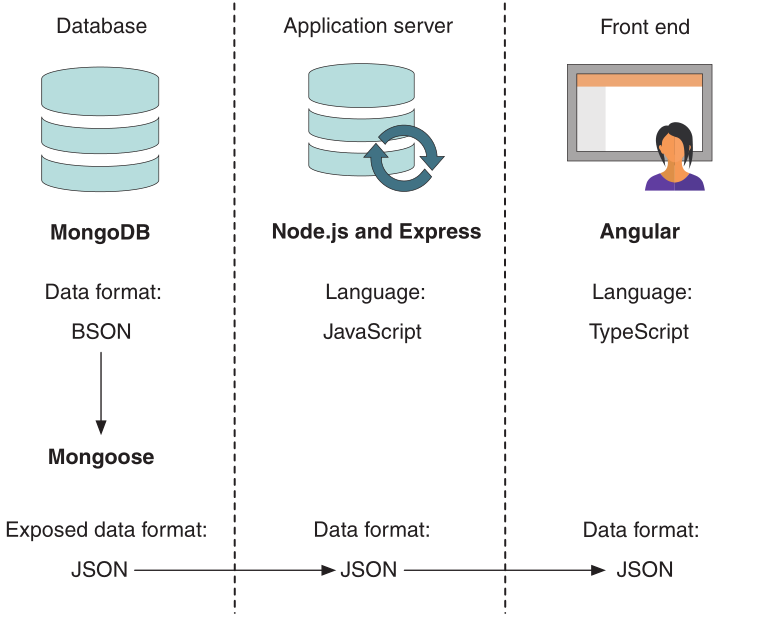
\includegraphics[scale=0.60]{assets/mean.png}
    \caption{Mean Stack}
    \label{fig:mean}
\end{figure}

\section{Model View Controller Design Pattern}

The Model View Controller (MVC) design pattern specifies that an application consist of a data model, presentation information, and control information. The pattern requires that each of these be separated into different objects.

MVC is more of an architectural pattern, but not for complete application. MVC mostly relates to the UI / interaction layer of an application. We’re still going to need business logic layer, maybe some service layer and data access layer.



\begin{enumerate}
    \item Model contains only the pure application data, it contains no logic describing how to present the data to a user.
    \item View presents the model’s data to the user. The view knows how to access the model’s data, but it does not know what this data means or what the user can do to manipulate it.
    \item Controller exists between the view and the model. It listens to events triggered by the view (or another external source) and executes the appropriate reaction to these events. In most cases, the reaction is to call a method on the model. Since the view and the model are connected through a notification mechanism, the result of this action is then automatically reflected in the view.
\end{enumerate}

\begin{figure}[!ht]
    \center
    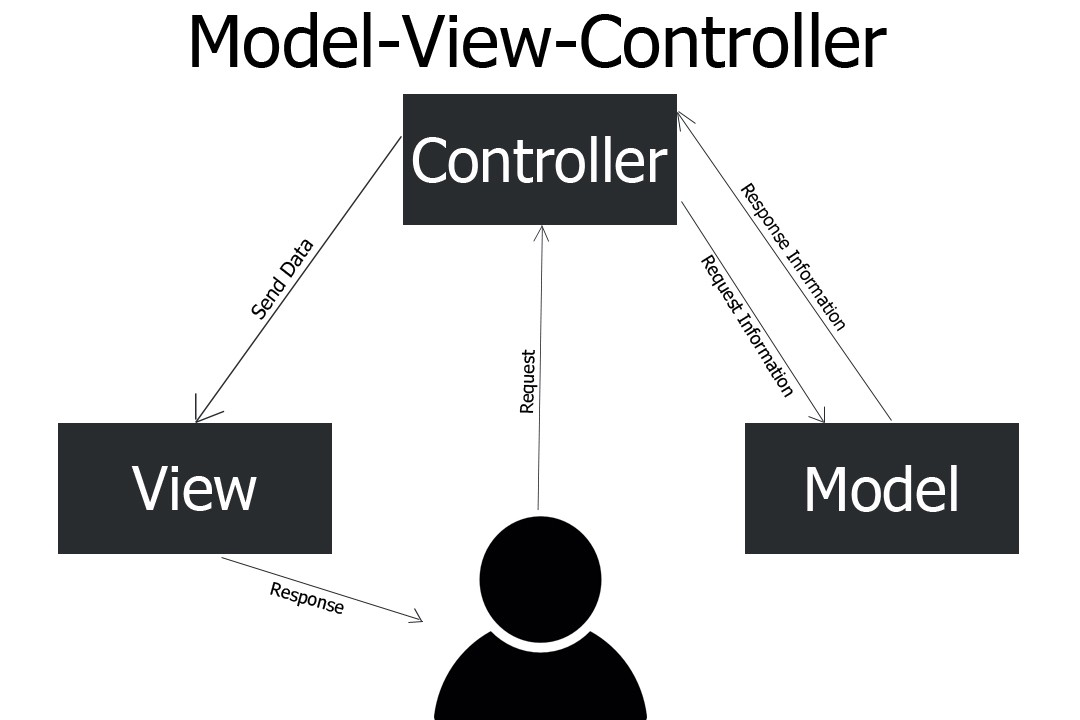
\includegraphics[scale=0.30]{assets/mvc.jpg}
    \caption{Model View Controller}
    \label{fig:mvc}
\end{figure}

\section{Representational State Transfer Architecture}
REST, or REpresentational State Transfer, is an architectural style for providing standards between computer systems on the web, making it easier for systems to communicate with each other. REST-compliant systems, often called RESTful systems, are characterized by how they are stateless and separate the concerns of client and server. We will go into what these terms mean and why they are beneficial characteristics for services on the Web.




\section{Software as a Service}
Software as a Service or SaaS , which allows us to set up services, such as application servers and databases, as needed to create the apps we need. This type of system typically works in a cloud or hybrid cloud environment, which often makes provisioning of servers and software as simple as entering some configurations and clicking a button.

This type of setup is perfect for the MEAN stack, as each piece of the MEAN stack is easily placed into the cloud and thus can be easily provisioned, so they are widely available on SaaS services and can be used quickly when needed. If we are looking for a good development stack, the MEAN stack has much to offer for IT management as well as for developers!



\section{Monolithic Applications}

If all the functionalities of a project exists in a single codebase, then that application is known as monolithic application. We all must have designed a monolithic application in our lives in which we were given a problem statement and were asked to design a system with various functionalities. We design our application in various layers like presentation, service and persistence and then deploy that codebase as single jar/war file. This is nothing but a monolithic application where “mono” represents the single codebase containing all the required functionalities.
\begin{figure}[!ht]
    \center
    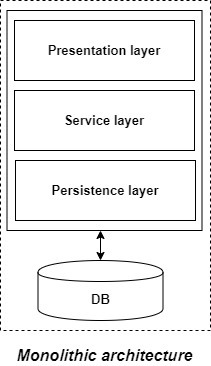
\includegraphics[scale=0.60]{assets/monolithic.jpg}
    \caption{Monolithic Applications}
    \label{fig:monoapp}
\end{figure}

Disadvantages of Monolithic applications:
\begin{enumerate}
    \item
          It becomes too large in size with time and hence, difficult to manage.
    \item
          We need to redeploy the whole application even for a small change.
    \item
          As the size of the application increases, its start-up and deployment time also increases.
    \item
          For any new developer joining the project, it is very difficult to understand the logic of large Monolithic application even if his responsibility is related to a single functionality.
    \item
          Even if a single part of the application is facing a large load/traffic, we need to deploy the instances of the whole application in multiple servers. It is very inefficient and takes up more resources unnecessarily. Hence, horizontal scaling is not feasible in monolithic applications.
    \item
          It is very difficult to adopt any new technology which is well suited for a particular functionality as it affects the whole application, both in terms of time and cost.
    \item
          It is not very reliable as a single bug in any module can bring down the whole monolithic application.
\end{enumerate}
Advantages of monolithic applications:
\begin{enumerate}
    \item
          Simple to develop relative to microservices where skilled developers are required in order to identify and develop the services.
    \item
          Easier to deploy as only a single jar/war file is deployed.
    \item
          Relatively easier and simple to develop in comparison to microservices architecture.
    \item
          The problems of network latency and security are relatively less in comparison to microservices architecture.
\end{enumerate}


\section{Conception}
\subsection{Unified Modeling Language}
\subsection{PlantUml}
PlantUML is an open-source tool allowing users to create UML diagrams from a plain text language. The language of PlantUML is an example of a Domain-specific language. It uses Graphviz software to lay out its diagrams. It has been used to allow blind students to work with UML. PlantUML also helps blind software engineers to design and read UML diagrams.


\subsection{Gantt chart}
A gantt chart is a horizontal bar chart that visually represents a project plan over time. Modern gantt charts typically show us the status of—as well as who’s responsible for—each task in the project.

In other words, a gantt chart is a super-simple way to keep us out of a project pinch!

What are the key parts of a gantt chart?
A gantt chart is made up of several different elements:
\begin{enumerate}
    \item
          Task list: Runs vertically down the left of the gantt chart to describe project work and may be organized into groups and subgroups
    \item
          Timeline: Runs horizontally across the top of the gantt chart and shows months, weeks, days, and years
    \item
          Dateline: A vertical line that highlights the current date on the gantt chart
    \item
          Bars: Horizontal markers on the right side of the gantt chart that represent tasks and show progress, duration, and start and end dates
    \item
          Milestones: Yellow diamonds that call out major events, dates, decisions, and deliverables
    \item
          Dependencies: Light gray lines that connect tasks that need to happen in a certain order
    \item
          Progress: Shows how far along work is and may be indicated by \% Complete and/or bar shading
    \item
          Resource assigned: Indicates the person or team responsible for completing a task
\end{enumerate}


\section{Design}
\subsection{Adobe Photoshop}
Adobe Photoshop is a software application for image editing and photo retouching for use on Windows or MacOS computers. Photoshop offers users the ability to create, enhance, or otherwise edit images, artwork, and illustrations. Changing backgrounds, simulating a real-life painting, or creating an alternative view of the universe are all possible with Adobe Photoshop. It is the most widely used software tool for photo editing, image manipulation, and retouching for numerous image and video file formats. The tools within Photoshop make it possible to edit both individual images as well as large batches of photos.
We used it to prototype and create our platform logo.
\subsection{Adobe XD}
Adobe XD is a vector-based user experience design tool for web apps and mobile apps, developed and published by Adobe Inc. It is available for macOS and Windows, although there are versions for iOS and Android to help preview the result of work directly on mobile devices. XD.


\section{Front-End}
We decided to go with the single page application instead of the multiple pages application and we will be using the following tools for the front end.
\subsection{HTML}
Hypertext Markup Language (HTML) is the standard markup language for documents designed to be displayed in a web browser. It can be assisted by technologies such as Cascading Style Sheets (CSS) and scripting languages such as JavaScript.

Web browsers receive HTML documents from a web server or from local storage and render the documents into multimedia web pages. HTML describes the structure of a web page semantically and originally included cues for the appearance of the document.



\subsection{CSS}
Cascading Style Sheets (CSS) is a style sheet language used for describing the presentation of a document written in a markup language like HTML.[1] CSS is a cornerstone technology of the World Wide Web, alongside HTML and JavaScript.[2]

CSS is designed to enable the separation of presentation and content, including layout, colors, and fonts.[3] This separation can improve content accessibility, provide more flexibility and control in the specification of presentation characteristics, enable multiple web pages to share formatting by specifying the relevant CSS in a separate .css file, and reduce complexity and repetition in the structural content.


\subsection{Typescript}
TypeScript is an open-source programming language developed and maintained by Microsoft. It is a strict syntactical superset of JavaScript and adds optional static typing to the language. TypeScript is designed for development of large applications and transcompiles to JavaScript.[5] As TypeScript is a superset of JavaScript, existing JavaScript programs are also valid TypeScript programs.

TypeScript may be used to develop JavaScript applications for both client-side and server-side execution (as with Node.js or Deno). There are multiple options available for transcompilation. Either the default TypeScript Checker can be used,[6] or the Babel compiler can be invoked to convert TypeScript to JavaScript.

TypeScript supports definition files that can contain type information of existing JavaScript libraries, much like C++ header files can describe the structure of existing object files. This enables other programs to use the values defined in the files as if they were statically typed TypeScript entities. There are third-party header files for popular libraries such as jQuery, MongoDB, and D3.js. TypeScript headers for the Node.js basic modules are also available, allowing development of Node.js programs within TypeScript.

The TypeScript compiler is itself written in TypeScript and compiled to JavaScript. It is licensed under the Apache License 2.0. TypeScript is included as a first-class programming language in Microsoft Visual Studio 2013 Update 2 and later, beside C\# and other Microsoft languages. An official extension allows Visual Studio 2012 to support TypeScript as well. Anders Hejlsberg, lead architect of C\# and creator of Delphi and Turbo Pascal, has worked on the development of TypeScript.



\subsection{Angular 9}
Angular is an app-design framework and development platform for creating efficient and sophisticated single-page apps in html, css, and Typescript which is a superset of JavaScript. Angular provides built-in features for animation, http service, and materials which in turn have features such as auto-complete, navigation, toolbar, menus, etc. The code is written in Typescript, which compiles to JavaScript and displays the same in the browser.
\subsection{Hypertext Transfer Protocol}
The Hypertext Transfer Protocol (HTTP) is an application protocol for distributed, collaborative, hypermedia information systems. HTTP is the foundation of data communication for the World Wide Web, where hypertext documents include hyperlinks to other resources that the user can easily access, for example by a mouse click or by tapping the screen in a web browser.
\subsection{JSON}
JavaScript Object Notation (JSON) is an open standard file format, and data interchange format, that uses human-readable text to store and transmit data objects consisting of attribute–value pairs and array data types (or any other serializable value). It is a very common data format, with a diverse range of applications, such as serving as a replacement for XML in AJAX systems.

JSON is a language-independent data format. It was derived from JavaScript, but many modern programming languages include code to generate and parse JSON-format data. The official Internet media type for JSON is application/json. JSON filenames use the extension .json.



\section{Back-End}
\subsection{Javascript}
JavaScript often abbreviated as JS, is a programming language that conforms to the ECMAScript specification.[7] JavaScript is high-level, often just-in-time compiled, and multi-paradigm. It has curly-bracket syntax, dynamic typing, prototype-based object-orientation, and first-class functions.


\subsection{Node Js}
Node.js is an open source, cross-platform runtime environment for developing server-side and networking applications. Node.js applications are written in JavaScript, and can be run within the Node.js runtime on OS X, Microsoft Windows, and Linux.
Node.js also provides a rich library of various JavaScript modules which simplifies the development of web applications using Node.js to a great extent.

Following are some of the important features that make Node.js the first choice of software architects.
\begin{enumerate}
    \item
          Asynchronous and Event Driven: All APIs of Node.js library are asynchronous, that is, non-blocking. It essentially means a Node.js based server never waits for an API to return data. The server moves to the next API after calling it and a notification mechanism of Events of Node.js helps the server to get a response from the previous API call.
    \item
          Very Fast: Being built on Google Chrome's V8 JavaScript Engine, Node.js library is very fast in code execution.
    \item
          Single Threaded but Highly Scalable: Node.js uses a single threaded model with event looping. Event mechanism helps the server to respond in a non-blocking way and makes the server highly scalable as opposed to traditional servers which create limited threads to handle requests. Node.js uses a single threaded program and the same program can provide service to a much larger number of requests than traditional servers like Apache HTTP Server.
    \item
          No Buffering: Node.js applications never buffer any data. These applications simply output the data in chunks.
    \item
          License: Node.js is released under the MIT license
\end{enumerate}





\subsection{Express Js}
ExpressJS is a web application framework that provides us with a simple API to build websites, web apps and back ends. With ExpressJS, we need not worry about low level protocols, processes, etc.
Express provides a minimal interface to build our applications. It provides us the tools that are required to build our app. It is flexible as there are numerous modules available on npm, which can be directly plugged into Express.
Express was developed by TJ Holowaychuk and is maintained by the Node.js foundation and numerous open source contributors.



\subsection{MongoDB}
MongoDB is a cross-platform, document oriented database that provides, high performance, high availability, and easy scalability. MongoDB works on concept of collection and document.
\begin{enumerate}
    \item
          Database\\
          Database is a physical container for collections. Each database gets its own set of files on the file system. A single MongoDB server typically has multiple databases.
    \item
          Collection\\
          Collection is a group of MongoDB documents. It is the equivalent of an RDBMS table. A collection exists within a single database. Collections do not enforce a schema. Documents within a collection can have different fields. Typically, all documents in a collection are of similar or related purpose.
    \item
          Document\\
          A document is a set of key-value pairs. Documents have dynamic schema. Dynamic schema means that documents in the same collection do not need to have the same set of fields or structure, and common fields in a collection's documents may hold different types of data.
\end{enumerate}





\subsection{Mongoose}
Mongoose is an Object Data Modeling (ODM) library for MongoDB and Node.js. It manages relationships between data, provides schema validation, and is used to translate between objects in code and the representation of those objects in MongoDB.


\section{Development}
\subsection{Visual Studio Code}
DescriptionVisual Studio Code is a source-code editor developed by Microsoft for Windows, Linux and macOS. It includes support for debugging, embedded Git control and GitHub, syntax highlighting, intelligent code completion, snippets, and code refactoring.


\subsection{MongoDB Compass Community}
MongoDB Compass is the defacto GUI tool for MongoDB much like MySQL Workbench is MySQL’s associated tool. It allows us to visually explore our data, run ad hoc queries, interact with our data with full CRUD functionality, as well as view and optimize our queries’ performance.



\subsection{Postman}
Postman is an interactive and automatic tool for verifying the APIs of our project. Postman is a Google Chrome app for interacting with HTTP APIs. It presents us with a friendly GUI for constructing requests and reading responses. It works on the backend, and makes sure that each API is working as intended.

In Postman, we create a request, and Postman looks at the response to make sure it has the element we want in it. As it is an automation tool, it drastically improves testing time and quality of the project. It helps in the early detection of bugs that might sprout at later stages and cause more damage to the system.

Postman is the way to streamline the process of API testing. All APIs that we create and deploy first rigorously go through Postman so that any major or show stopper bugs are identified on time and fewer bugs leak through to later stages.



\subsection{Git}
% Git is a version control system for tracking changes in computer files and coordinating work on those files among multiple people. It is primarily used for source code management in software development, but it can be used to keep track of changes in any set of files. As a distributed revision control system it is aimed at speed, data integrity, and support for distributed, non-linear workflows.
Git is a distributed revision control and source code management system that
allows several people to work on the same codebase at the same time on different
computers and networks. These can be pushed together, with all changes stored and
recorded. It’s also possible to roll back to an earlier state if necessary.
\subsection{Github}
At a high level, GitHub is a website and cloud-based service that helps developers store and manage their code, as well as track and control changes to their code. To understand exactly what GitHub is, we need to know two connected principles:
\begin{enumerate}
    \item Version control
    \item Git
\end{enumerate}

\subsection{Github Desktop}
GitHub Desktop is a fast and easy way to contribute to projects from Windows and OS X, whether we are a seasoned users or new users, GitHub Desktop is designed to simplify all processes and workflow in our GitHub. GitHub Desktop is an open-source Electron-based GitHub app. It is written in TypeScript and uses React.


\subsection{Boost Note}
% Boostnote is an Open source note-taking app for programmers.
% Boostnote is niche tool because designed for programmers, but we are passionate for it.
% It focuses on writing Markdown note and code snippet quickly, can organized in a better way.
% You can sync data to multi-devices(Mac, Windows, Linux, Android and iOS) via Dropbox.
% Boostnote is not an app suitable for everyone, it ‘s a handy note-taking app for programmers.
% Boostnote has two main features.
% Markdown note
% Since Boostnote is a Markdown editor, mainly write with markdown.
% Content is automatically saved while editing notes.
% Since preview could be viewed with one touch, you can immediately check the Markdown preview you are writing.
% Snippet note
% In the code snippet, you can highlight code syntax in over 100 languages ​​such as Javascript, Python, HTML, etc., and save multiple code snippets in one note.
% The indent and tab size can be set from the editor window.


\subsection{Latex}
\latex{} is a tool used to create professional-looking documents. It is based on the WYSIWYM (what we see is what we mean) idea, meaning we only have focus on the contents of our document and the computer will take care of the formatting. Instead of spacing out text on a page to control formatting, as with Microsoft Word or LibreOffice Writer, users can enter plain text and let LATEX take care of the rest.
\subsection{MiKTex}
% MiKTeX provides the tools necessary to prepare documents using the TeX/LaTeX markup language, as well as a simple tex editor: TeXworks.

\subsection{Tex Live}
% TeX Live is intended to be a straightforward way to get up and running with the TeX document production system. It provides a comprehensive TeX system with binaries for most flavors of Unix, including GNU/Linux, macOS, and also Windows. It includes all the major TeX-related programs, macro packages, and fonts that are free software, including support for many languages around the world. Many operating systems provide it via their own distributions.



\subsection{Markdown}
Markdown is a lightweight markup language with plain-text-formatting syntax. Its design allows it to be converted to many output formats, but the original tool by the same name only supports HTML. Markdown is often used to format readme files, for writing messages in online discussion forums, and to create rich text using a plain text editor.
\subsection{Marp}
Marp is the ecosystem to write our presentation with plain Markdown
\section{Deployment}
\subsection{Google Cloud Platform}
\subsection{MongoDB Atlas}


    % \cleardoublepage%

    % Back matter
    % @Author: Taha Bouhsine
\setcounter{mtc}{13}

\chapter*{Conclusion}
\label{chap:conclusion}
\minitoc
\markboth{\MakeUppercase{Conclusion}}{}%
\addcontentsline{toc}{chapter}{Conclusion}
  And a very interesting conclusion here\@. ~\\
  Lorem ipsum dolor sit amet, consectetur adipisicing elit, sed do eiusmod
  tempor incididunt ut labore et dolore magna aliqua. Ut enim ad minim veniam,
  quis nostrud exercitation ullamco laboris nisi ut aliquip ex ea commodo
  consequat. Duis aute irure dolor in reprehenderit in voluptate velit esse
  cillum dolore eu fugiat nulla pariatur. Excepteur sint occaecat cupidatat non
  proident, sunt in culpa qui officia deserunt mollit anim id est laborum.
  Lorem ipsum dolor sit amet, consectetur adipisicing elit, sed do eiusmod
  tempor incididunt ut labore et dolore magna aliqua. Ut enim ad minim veniam,
  quis nostrud exercitation ullamco laboris nisi ut aliquip ex ea commodo
  consequat. Duis aute irure dolor in reprehenderit in voluptate velit esse
  cillum dolore eu fugiat nulla pariatur. Excepteur sint occaecat cupidatat non
  proident, sunt in culpa qui officia deserunt mollit anim id est laborum.
    \cleardoublepage%

    % @Author: Taha Bouhsine
\setcounter{mtc}{12}

\chapter*{Appendix}
\label{chap:appendix}
\minitoc
\markboth{\MakeUppercase{Appendix}}{}
\addcontentsline{toc}{chapter}{Appendix}
\section*{Use cases Description}
\label{sec:ucd}

\begin{table}[H]

  \centering
  \def\arraystretch{1.5}


  \begin{tabularx}{\linewidth}{|l|X|X|X|}

    \hline Use Case \#1                  & \multicolumn{3} {l|}{Register}                                                                        \\ \hline Goal in
    Description                          & \multicolumn{3}{>{\hsize=\dimexpr 3\hsize+4\tabcolsep+2\arrayrulewidth\relax}X|}{                     %
      This is a very long line. Lorem ipsum dolor sit amet, consectetur
      adipiscing elit, sed do eiusmod tempor incididunt ut labore et
      dolore magna aliqua.  }                                                                                                                    \\
    \hline Stereotype and Package        &
    \multicolumn{3}{l|}{}                                                                                                                        \\
    \hline Preconditions                 &
    \multicolumn{3}{l|}{}                                                                                                                        \\
    \hline Postconditions                &
    \multicolumn{3}{l|}{}                                                                                                                        \\
    \hline Primary Actors                &
    \multicolumn{3}{l|}{}                                                                                                                        \\
    \hline Use Case Relationships:       &
    \multicolumn{3}{l|}{}                                                                                                                        \\
    \hline Basic Flow                    &
    \multicolumn{3}{l|}{}                                                                                                                        \\
    \hline Alternative Flow              & \multicolumn{3}{l|}{}                                                                                 \\


    \hline Exceptions                    & \multicolumn{3}{l|}{}                                                                                 \\

    \hline Constraints                   & \multicolumn{3}{l|}{}                                                                                 \\

    \hline User Interface Specifications & \multicolumn{3}{l|}{}                                                                                 \\

    \hline \multirow{2}{*}{}             & Metrics                                                                           & Priority & Status \\
    \cline{2-4}                          &                                                                                   &          &        \\
    \hline Notes                         & \multicolumn{3}{l|}{}                                                                                 \\
    \hline
  \end{tabularx}
  \caption{Use Case Register}
  \label{tab:use_case_register}
\end{table}

\begin{table}[H]

  \centering
  \def\arraystretch{1.5}


  \begin{tabularx}{\linewidth}{|l|X|X|X|}

    \hline Use Case \#2                  & \multicolumn{3} {l|}{Login}                                                                           \\ \hline Goal in
    Description                          & \multicolumn{3}{>{\hsize=\dimexpr 3\hsize+4\tabcolsep+2\arrayrulewidth\relax}X|}{                     %
      This is a very long line. Lorem ipsum dolor sit amet, consectetur
      adipiscing elit, sed do eiusmod tempor incididunt ut labore et
      dolore magna aliqua.  }                                                                                                                    \\
    \hline Stereotype and Package        &
    \multicolumn{3}{l|}{}                                                                                                                        \\
    \hline Preconditions                 &
    \multicolumn{3}{l|}{}                                                                                                                        \\
    \hline Postconditions                &
    \multicolumn{3}{l|}{}                                                                                                                        \\
    \hline Primary Actors                &
    \multicolumn{3}{l|}{}                                                                                                                        \\
    \hline Use Case Relationships:       &
    \multicolumn{3}{l|}{}                                                                                                                        \\
    \hline Basic Flow                    &
    \multicolumn{3}{l|}{}                                                                                                                        \\
    \hline Alternative Flow              & \multicolumn{3}{l|}{}                                                                                 \\


    \hline Exceptions                    & \multicolumn{3}{l|}{}                                                                                 \\

    \hline Constraints                   & \multicolumn{3}{l|}{}                                                                                 \\

    \hline User Interface Specifications & \multicolumn{3}{l|}{}                                                                                 \\

    \hline \multirow{2}{*}{}             & Metrics                                                                           & Priority & Status \\
    \cline{2-4}                          &                                                                                   &          &        \\
    \hline Notes                         & \multicolumn{3}{l|}{}                                                                                 \\
    \hline
  \end{tabularx}
  \caption{Use Case Login}
  \label{tab:use_case_login}
\end{table}

\begin{table}[H]

  \centering
  \def\arraystretch{1.5}


  \begin{tabularx}{\linewidth}{|l|X|X|X|}

    \hline Use Case \#3                  & \multicolumn{3} {l|}{Reset Password}                                                                  \\ \hline Goal in
    Description                          & \multicolumn{3}{>{\hsize=\dimexpr 3\hsize+4\tabcolsep+2\arrayrulewidth\relax}X|}{                     %
      This is a very long line. Lorem ipsum dolor sit amet, consectetur
      adipiscing elit, sed do eiusmod tempor incididunt ut labore et
      dolore magna aliqua.  }                                                                                                                    \\
    \hline Stereotype and Package        &
    \multicolumn{3}{l|}{}                                                                                                                        \\
    \hline Preconditions                 &
    \multicolumn{3}{l|}{}                                                                                                                        \\
    \hline Postconditions                &
    \multicolumn{3}{l|}{}                                                                                                                        \\
    \hline Primary Actors                &
    \multicolumn{3}{l|}{}                                                                                                                        \\
    \hline Use Case Relationships:       &
    \multicolumn{3}{l|}{}                                                                                                                        \\
    \hline Basic Flow                    &
    \multicolumn{3}{l|}{}                                                                                                                        \\
    \hline Alternative Flow              & \multicolumn{3}{l|}{}                                                                                 \\


    \hline Exceptions                    & \multicolumn{3}{l|}{}                                                                                 \\

    \hline Constraints                   & \multicolumn{3}{l|}{}                                                                                 \\

    \hline User Interface Specifications & \multicolumn{3}{l|}{}                                                                                 \\

    \hline \multirow{2}{*}{}             & Metrics                                                                           & Priority & Status \\
    \cline{2-4}                          &                                                                                   &          &        \\
    \hline Notes                         & \multicolumn{3}{l|}{}                                                                                 \\
    \hline
  \end{tabularx}
  \caption{Use Case Reset Password}
  \label{tab:use_case_reset_password}
\end{table}

\begin{table}[H]

  \centering
  \def\arraystretch{1.5}


  \begin{tabularx}{\linewidth}{|l|X|X|X|}

    \hline Use Case \#4                  & \multicolumn{3} {l|}{Change password}                                                                 \\ \hline Goal in
    Description                          & \multicolumn{3}{>{\hsize=\dimexpr 3\hsize+4\tabcolsep+2\arrayrulewidth\relax}X|}{                     %
      This is a very long line. Lorem ipsum dolor sit amet, consectetur
      adipiscing elit, sed do eiusmod tempor incididunt ut labore et
      dolore magna aliqua.  }                                                                                                                    \\
    \hline Stereotype and Package        &
    \multicolumn{3}{l|}{}                                                                                                                        \\
    \hline Preconditions                 &
    \multicolumn{3}{l|}{}                                                                                                                        \\
    \hline Postconditions                &
    \multicolumn{3}{l|}{}                                                                                                                        \\
    \hline Primary Actors                &
    \multicolumn{3}{l|}{}                                                                                                                        \\
    \hline Use Case Relationships:       &
    \multicolumn{3}{l|}{}                                                                                                                        \\
    \hline Basic Flow                    &
    \multicolumn{3}{l|}{}                                                                                                                        \\
    \hline Alternative Flow              & \multicolumn{3}{l|}{}                                                                                 \\


    \hline Exceptions                    & \multicolumn{3}{l|}{}                                                                                 \\

    \hline Constraints                   & \multicolumn{3}{l|}{}                                                                                 \\

    \hline User Interface Specifications & \multicolumn{3}{l|}{}                                                                                 \\

    \hline \multirow{2}{*}{}             & Metrics                                                                           & Priority & Status \\
    \cline{2-4}                          &                                                                                   &          &        \\
    \hline Notes                         & \multicolumn{3}{l|}{}                                                                                 \\
    \hline
  \end{tabularx}
  \caption{Use Case Change password}
  \label{tab:use_case_change_password}
\end{table}

\begin{table}[H]

  \centering
  \def\arraystretch{1.5}


  \begin{tabularx}{\linewidth}{|l|X|X|X|}

    \hline Use Case \#5                  & \multicolumn{3} {l|}{Logout}                                                                          \\ \hline Goal in
    Description                          & \multicolumn{3}{>{\hsize=\dimexpr 3\hsize+4\tabcolsep+2\arrayrulewidth\relax}X|}{                     %
      This is a very long line. Lorem ipsum dolor sit amet, consectetur
      adipiscing elit, sed do eiusmod tempor incididunt ut labore et
      dolore magna aliqua.  }                                                                                                                    \\
    \hline Stereotype and Package        &
    \multicolumn{3}{l|}{}                                                                                                                        \\
    \hline Preconditions                 &
    \multicolumn{3}{l|}{}                                                                                                                        \\
    \hline Postconditions                &
    \multicolumn{3}{l|}{}                                                                                                                        \\
    \hline Primary Actors                &
    \multicolumn{3}{l|}{}                                                                                                                        \\
    \hline Use Case Relationships:       &
    \multicolumn{3}{l|}{}                                                                                                                        \\
    \hline Basic Flow                    &
    \multicolumn{3}{l|}{}                                                                                                                        \\
    \hline Alternative Flow              & \multicolumn{3}{l|}{}                                                                                 \\


    \hline Exceptions                    & \multicolumn{3}{l|}{}                                                                                 \\

    \hline Constraints                   & \multicolumn{3}{l|}{}                                                                                 \\

    \hline User Interface Specifications & \multicolumn{3}{l|}{}                                                                                 \\

    \hline \multirow{2}{*}{}             & Metrics                                                                           & Priority & Status \\
    \cline{2-4}                          &                                                                                   &          &        \\
    \hline Notes                         & \multicolumn{3}{l|}{}                                                                                 \\
    \hline
  \end{tabularx}
  \caption{Use Case Logout}
  \label{tab:use_case_logout}
\end{table}

\begin{table}[H]

  \centering
  \def\arraystretch{1.5}


  \begin{tabularx}{\linewidth}{|l|X|X|X|}

    \hline Use Case \#6                  & \multicolumn{3} {l|}{Role management}                                                                 \\ \hline Goal in
    Description                          & \multicolumn{3}{>{\hsize=\dimexpr 3\hsize+4\tabcolsep+2\arrayrulewidth\relax}X|}{                     %
      This is a very long line. Lorem ipsum dolor sit amet, consectetur
      adipiscing elit, sed do eiusmod tempor incididunt ut labore et
      dolore magna aliqua.  }                                                                                                                    \\
    \hline Stereotype and Package        &
    \multicolumn{3}{l|}{}                                                                                                                        \\
    \hline Preconditions                 &
    \multicolumn{3}{l|}{}                                                                                                                        \\
    \hline Postconditions                &
    \multicolumn{3}{l|}{}                                                                                                                        \\
    \hline Primary Actors                &
    \multicolumn{3}{l|}{}                                                                                                                        \\
    \hline Use Case Relationships:       &
    \multicolumn{3}{l|}{}                                                                                                                        \\
    \hline Basic Flow                    &
    \multicolumn{3}{l|}{}                                                                                                                        \\
    \hline Alternative Flow              & \multicolumn{3}{l|}{}                                                                                 \\


    \hline Exceptions                    & \multicolumn{3}{l|}{}                                                                                 \\

    \hline Constraints                   & \multicolumn{3}{l|}{}                                                                                 \\

    \hline User Interface Specifications & \multicolumn{3}{l|}{}                                                                                 \\

    \hline \multirow{2}{*}{}             & Metrics                                                                           & Priority & Status \\
    \cline{2-4}                          &                                                                                   &          &        \\
    \hline Notes                         & \multicolumn{3}{l|}{}                                                                                 \\
    \hline
  \end{tabularx}
  \caption{Use Case Role management}
  \label{tab:use_case_role_management}
\end{table}

\begin{table}[H]

  \centering
  \def\arraystretch{1.5}


  \begin{tabularx}{\linewidth}{|l|X|X|X|}

    \hline Use Case \#7                  & \multicolumn{3} {l|}{Send Payment}                                                                    \\ \hline Goal in
    Description                          & \multicolumn{3}{>{\hsize=\dimexpr 3\hsize+4\tabcolsep+2\arrayrulewidth\relax}X|}{                     %
      This is a very long line. Lorem ipsum dolor sit amet, consectetur
      adipiscing elit, sed do eiusmod tempor incididunt ut labore et
      dolore magna aliqua.  }                                                                                                                    \\
    \hline Stereotype and Package        &
    \multicolumn{3}{l|}{}                                                                                                                        \\
    \hline Preconditions                 &
    \multicolumn{3}{l|}{}                                                                                                                        \\
    \hline Postconditions                &
    \multicolumn{3}{l|}{}                                                                                                                        \\
    \hline Primary Actors                &
    \multicolumn{3}{l|}{}                                                                                                                        \\
    \hline Use Case Relationships:       &
    \multicolumn{3}{l|}{}                                                                                                                        \\
    \hline Basic Flow                    &
    \multicolumn{3}{l|}{}                                                                                                                        \\
    \hline Alternative Flow              & \multicolumn{3}{l|}{}                                                                                 \\


    \hline Exceptions                    & \multicolumn{3}{l|}{}                                                                                 \\

    \hline Constraints                   & \multicolumn{3}{l|}{}                                                                                 \\

    \hline User Interface Specifications & \multicolumn{3}{l|}{}                                                                                 \\

    \hline \multirow{2}{*}{}             & Metrics                                                                           & Priority & Status \\
    \cline{2-4}                          &                                                                                   &          &        \\
    \hline Notes                         & \multicolumn{3}{l|}{}                                                                                 \\
    \hline
  \end{tabularx}
  \caption{Use Case Send Payment}
  \label{tab:use_case_send_payment}
\end{table}

\begin{table}[H]

  \centering
  \def\arraystretch{1.5}


  \begin{tabularx}{\linewidth}{|l|X|X|X|}

    \hline Use Case \#8                  & \multicolumn{3} {l|}{Withdraw Payment}                                                                \\ \hline Goal in
    Description                          & \multicolumn{3}{>{\hsize=\dimexpr 3\hsize+4\tabcolsep+2\arrayrulewidth\relax}X|}{                     %
      This is a very long line. Lorem ipsum dolor sit amet, consectetur
      adipiscing elit, sed do eiusmod tempor incididunt ut labore et
      dolore magna aliqua.  }                                                                                                                    \\
    \hline Stereotype and Package        &
    \multicolumn{3}{l|}{}                                                                                                                        \\
    \hline Preconditions                 &
    \multicolumn{3}{l|}{}                                                                                                                        \\
    \hline Postconditions                &
    \multicolumn{3}{l|}{}                                                                                                                        \\
    \hline Primary Actors                &
    \multicolumn{3}{l|}{}                                                                                                                        \\
    \hline Use Case Relationships:       &
    \multicolumn{3}{l|}{}                                                                                                                        \\
    \hline Basic Flow                    &
    \multicolumn{3}{l|}{}                                                                                                                        \\
    \hline Alternative Flow              & \multicolumn{3}{l|}{}                                                                                 \\


    \hline Exceptions                    & \multicolumn{3}{l|}{}                                                                                 \\

    \hline Constraints                   & \multicolumn{3}{l|}{}                                                                                 \\

    \hline User Interface Specifications & \multicolumn{3}{l|}{}                                                                                 \\

    \hline \multirow{2}{*}{}             & Metrics                                                                           & Priority & Status \\
    \cline{2-4}                          &                                                                                   &          &        \\
    \hline Notes                         & \multicolumn{3}{l|}{}                                                                                 \\
    \hline
  \end{tabularx}
  \caption{Use Case withdraw Payment}
  \label{tab:use_case_withdraw_payment}
\end{table}

\begin{table}[H]

  \centering
  \def\arraystretch{1.5}


  \begin{tabularx}{\linewidth}{|l|X|X|X|}

    \hline Use Case \#9                  & \multicolumn{3} {l|}{Save the database}                                                               \\ \hline Goal in
    Description                          & \multicolumn{3}{>{\hsize=\dimexpr 3\hsize+4\tabcolsep+2\arrayrulewidth\relax}X|}{                     %
      This is a very long line. Lorem ipsum dolor sit amet, consectetur
      adipiscing elit, sed do eiusmod tempor incididunt ut labore et
      dolore magna aliqua.  }                                                                                                                    \\
    \hline Stereotype and Package        &
    \multicolumn{3}{l|}{}                                                                                                                        \\
    \hline Preconditions                 &
    \multicolumn{3}{l|}{}                                                                                                                        \\
    \hline Postconditions                &
    \multicolumn{3}{l|}{}                                                                                                                        \\
    \hline Primary Actors                &
    \multicolumn{3}{l|}{}                                                                                                                        \\
    \hline Use Case Relationships:       &
    \multicolumn{3}{l|}{}                                                                                                                        \\
    \hline Basic Flow                    &
    \multicolumn{3}{l|}{}                                                                                                                        \\
    \hline Alternative Flow              & \multicolumn{3}{l|}{}                                                                                 \\


    \hline Exceptions                    & \multicolumn{3}{l|}{}                                                                                 \\

    \hline Constraints                   & \multicolumn{3}{l|}{}                                                                                 \\

    \hline User Interface Specifications & \multicolumn{3}{l|}{}                                                                                 \\

    \hline \multirow{2}{*}{}             & Metrics                                                                           & Priority & Status \\
    \cline{2-4}                          &                                                                                   &          &        \\
    \hline Notes                         & \multicolumn{3}{l|}{}                                                                                 \\
    \hline
  \end{tabularx}
  \caption{Use Case Save the database}
  \label{tab:use_case_save_the_database}
\end{table}

\begin{table}[H]

  \centering
  \def\arraystretch{1.5}


  \begin{tabularx}{\linewidth}{|l|X|X|X|}

    \hline Use Case \#10                 & \multicolumn{3} {l|}{Restore the database}                                                            \\ \hline Goal in
    Description                          & \multicolumn{3}{>{\hsize=\dimexpr 3\hsize+4\tabcolsep+2\arrayrulewidth\relax}X|}{                     %
      This is a very long line. Lorem ipsum dolor sit amet, consectetur
      adipiscing elit, sed do eiusmod tempor incididunt ut labore et
      dolore magna aliqua.  }                                                                                                                    \\
    \hline Stereotype and Package        &
    \multicolumn{3}{l|}{}                                                                                                                        \\
    \hline Preconditions                 &
    \multicolumn{3}{l|}{}                                                                                                                        \\
    \hline Postconditions                &
    \multicolumn{3}{l|}{}                                                                                                                        \\
    \hline Primary Actors                &
    \multicolumn{3}{l|}{}                                                                                                                        \\
    \hline Use Case Relationships:       &
    \multicolumn{3}{l|}{}                                                                                                                        \\
    \hline Basic Flow                    &
    \multicolumn{3}{l|}{}                                                                                                                        \\
    \hline Alternative Flow              & \multicolumn{3}{l|}{}                                                                                 \\


    \hline Exceptions                    & \multicolumn{3}{l|}{}                                                                                 \\

    \hline Constraints                   & \multicolumn{3}{l|}{}                                                                                 \\

    \hline User Interface Specifications & \multicolumn{3}{l|}{}                                                                                 \\

    \hline \multirow{2}{*}{}             & Metrics                                                                           & Priority & Status \\
    \cline{2-4}                          &                                                                                   &          &        \\
    \hline Notes                         & \multicolumn{3}{l|}{}                                                                                 \\
    \hline
  \end{tabularx}
  \caption{Use Case Restore the database}
  \label{tab:use_case_restore_the_database}
\end{table}

\begin{table}[H]

  \centering
  \def\arraystretch{1.5}


  \begin{tabularx}{\linewidth}{|l|X|X|X|}

    \hline Use Case \#11                 & \multicolumn{3} {l|}{Dynamic data dispaly}                                                            \\ \hline Goal in
    Description                          & \multicolumn{3}{>{\hsize=\dimexpr 3\hsize+4\tabcolsep+2\arrayrulewidth\relax}X|}{                     %
      This is a very long line. Lorem ipsum dolor sit amet, consectetur
      adipiscing elit, sed do eiusmod tempor incididunt ut labore et
      dolore magna aliqua.  }                                                                                                                    \\
    \hline Stereotype and Package        &
    \multicolumn{3}{l|}{}                                                                                                                        \\
    \hline Preconditions                 &
    \multicolumn{3}{l|}{}                                                                                                                        \\
    \hline Postconditions                &
    \multicolumn{3}{l|}{}                                                                                                                        \\
    \hline Primary Actors                &
    \multicolumn{3}{l|}{}                                                                                                                        \\
    \hline Use Case Relationships:       &
    \multicolumn{3}{l|}{}                                                                                                                        \\
    \hline Basic Flow                    &
    \multicolumn{3}{l|}{}                                                                                                                        \\
    \hline Alternative Flow              & \multicolumn{3}{l|}{}                                                                                 \\


    \hline Exceptions                    & \multicolumn{3}{l|}{}                                                                                 \\

    \hline Constraints                   & \multicolumn{3}{l|}{}                                                                                 \\

    \hline User Interface Specifications & \multicolumn{3}{l|}{}                                                                                 \\

    \hline \multirow{2}{*}{}             & Metrics                                                                           & Priority & Status \\
    \cline{2-4}                          &                                                                                   &          &        \\
    \hline Notes                         & \multicolumn{3}{l|}{}                                                                                 \\
    \hline
  \end{tabularx}
  \caption{Use Case Dynamic data dispaly}
  \label{tab:use_case_dynamic_data_dispaly}
\end{table}

\begin{table}[H]

  \centering
  \def\arraystretch{1.5}


  \begin{tabularx}{\linewidth}{|l|X|X|X|}

    \hline Use Case \#12                 & \multicolumn{3} {l|}{Simultaneous updates}                                                            \\ \hline Goal in
    Description                          & \multicolumn{3}{>{\hsize=\dimexpr 3\hsize+4\tabcolsep+2\arrayrulewidth\relax}X|}{                     %
      This is a very long line. Lorem ipsum dolor sit amet, consectetur
      adipiscing elit, sed do eiusmod tempor incididunt ut labore et
      dolore magna aliqua.  }                                                                                                                    \\
    \hline Stereotype and Package        &
    \multicolumn{3}{l|}{}                                                                                                                        \\
    \hline Preconditions                 &
    \multicolumn{3}{l|}{}                                                                                                                        \\
    \hline Postconditions                &
    \multicolumn{3}{l|}{}                                                                                                                        \\
    \hline Primary Actors                &
    \multicolumn{3}{l|}{}                                                                                                                        \\
    \hline Use Case Relationships:       &
    \multicolumn{3}{l|}{}                                                                                                                        \\
    \hline Basic Flow                    &
    \multicolumn{3}{l|}{}                                                                                                                        \\
    \hline Alternative Flow              & \multicolumn{3}{l|}{}                                                                                 \\


    \hline Exceptions                    & \multicolumn{3}{l|}{}                                                                                 \\

    \hline Constraints                   & \multicolumn{3}{l|}{}                                                                                 \\

    \hline User Interface Specifications & \multicolumn{3}{l|}{}                                                                                 \\

    \hline \multirow{2}{*}{}             & Metrics                                                                           & Priority & Status \\
    \cline{2-4}                          &                                                                                   &          &        \\
    \hline Notes                         & \multicolumn{3}{l|}{}                                                                                 \\
    \hline
  \end{tabularx}
  \caption{Use Case Simultaneous updates}
  \label{tab:use_case_simultaneous_updates}
\end{table}

\begin{table}[H]

  \centering
  \def\arraystretch{1.5}


  \begin{tabularx}{\linewidth}{|l|X|X|X|}

    \hline Use Case \#13                 & \multicolumn{3} {l|}{Network deployment}                                                              \\ \hline Goal in
    Description                          & \multicolumn{3}{>{\hsize=\dimexpr 3\hsize+4\tabcolsep+2\arrayrulewidth\relax}X|}{                     %
      This is a very long line. Lorem ipsum dolor sit amet, consectetur
      adipiscing elit, sed do eiusmod tempor incididunt ut labore et
      dolore magna aliqua.  }                                                                                                                    \\
    \hline Stereotype and Package        &
    \multicolumn{3}{l|}{}                                                                                                                        \\
    \hline Preconditions                 &
    \multicolumn{3}{l|}{}                                                                                                                        \\
    \hline Postconditions                &
    \multicolumn{3}{l|}{}                                                                                                                        \\
    \hline Primary Actors                &
    \multicolumn{3}{l|}{}                                                                                                                        \\
    \hline Use Case Relationships:       &
    \multicolumn{3}{l|}{}                                                                                                                        \\
    \hline Basic Flow                    &
    \multicolumn{3}{l|}{}                                                                                                                        \\
    \hline Alternative Flow              & \multicolumn{3}{l|}{}                                                                                 \\


    \hline Exceptions                    & \multicolumn{3}{l|}{}                                                                                 \\

    \hline Constraints                   & \multicolumn{3}{l|}{}                                                                                 \\

    \hline User Interface Specifications & \multicolumn{3}{l|}{}                                                                                 \\

    \hline \multirow{2}{*}{}             & Metrics                                                                           & Priority & Status \\
    \cline{2-4}                          &                                                                                   &          &        \\
    \hline Notes                         & \multicolumn{3}{l|}{}                                                                                 \\
    \hline
  \end{tabularx}
  \caption{Use Case Network deployment}
  \label{tab:use_case_network_deployment}
\end{table}

\begin{table}[H]

  \centering
  \def\arraystretch{1.5}


  \begin{tabularx}{\linewidth}{|l|X|X|X|}

    \hline Use Case \#14                 & \multicolumn{3} {l|}{Run on different browsers and platforms}                                         \\ \hline Goal in
    Description                          & \multicolumn{3}{>{\hsize=\dimexpr 3\hsize+4\tabcolsep+2\arrayrulewidth\relax}X|}{                     %
      This is a very long line. Lorem ipsum dolor sit amet, consectetur
      adipiscing elit, sed do eiusmod tempor incididunt ut labore et
      dolore magna aliqua.  }                                                                                                                    \\
    \hline Stereotype and Package        &
    \multicolumn{3}{l|}{}                                                                                                                        \\
    \hline Preconditions                 &
    \multicolumn{3}{l|}{}                                                                                                                        \\
    \hline Postconditions                &
    \multicolumn{3}{l|}{}                                                                                                                        \\
    \hline Primary Actors                &
    \multicolumn{3}{l|}{}                                                                                                                        \\
    \hline Use Case Relationships:       &
    \multicolumn{3}{l|}{}                                                                                                                        \\
    \hline Basic Flow                    &
    \multicolumn{3}{l|}{}                                                                                                                        \\
    \hline Alternative Flow              & \multicolumn{3}{l|}{}                                                                                 \\


    \hline Exceptions                    & \multicolumn{3}{l|}{}                                                                                 \\

    \hline Constraints                   & \multicolumn{3}{l|}{}                                                                                 \\

    \hline User Interface Specifications & \multicolumn{3}{l|}{}                                                                                 \\

    \hline \multirow{2}{*}{}             & Metrics                                                                           & Priority & Status \\
    \cline{2-4}                          &                                                                                   &          &        \\
    \hline Notes                         & \multicolumn{3}{l|}{}                                                                                 \\
    \hline
  \end{tabularx}
  \caption{Use Case Run on different browsers and platforms}
  \label{tab:use_case_multi_platform}
\end{table}

\begin{table}[H]

  \centering
  \def\arraystretch{1.5}


  \begin{tabularx}{\linewidth}{|l|X|X|X|}

    \hline Use Case \#15                 & \multicolumn{3} {l|}{CRUD Fundraisers}                                                                \\ \hline Goal in
    Description                          & \multicolumn{3}{>{\hsize=\dimexpr 3\hsize+4\tabcolsep+2\arrayrulewidth\relax}X|}{                     %
      This is a very long line. Lorem ipsum dolor sit amet, consectetur
      adipiscing elit, sed do eiusmod tempor incididunt ut labore et
      dolore magna aliqua.  }                                                                                                                    \\
    \hline Stereotype and Package        &
    \multicolumn{3}{l|}{}                                                                                                                        \\
    \hline Preconditions                 &
    \multicolumn{3}{l|}{}                                                                                                                        \\
    \hline Postconditions                &
    \multicolumn{3}{l|}{}                                                                                                                        \\
    \hline Primary Actors                &
    \multicolumn{3}{l|}{}                                                                                                                        \\
    \hline Use Case Relationships:       &
    \multicolumn{3}{l|}{}                                                                                                                        \\
    \hline Basic Flow                    &
    \multicolumn{3}{l|}{}                                                                                                                        \\
    \hline Alternative Flow              & \multicolumn{3}{l|}{}                                                                                 \\


    \hline Exceptions                    & \multicolumn{3}{l|}{}                                                                                 \\

    \hline Constraints                   & \multicolumn{3}{l|}{}                                                                                 \\

    \hline User Interface Specifications & \multicolumn{3}{l|}{}                                                                                 \\

    \hline \multirow{2}{*}{}             & Metrics                                                                           & Priority & Status \\
    \cline{2-4}                          &                                                                                   &          &        \\
    \hline Notes                         & \multicolumn{3}{l|}{}                                                                                 \\
    \hline
  \end{tabularx}
  \caption{Use Case CRUD Fundraisers}
  \label{tab:use_case_fundraisers_crud}
\end{table}




\begin{table}[H]

  \centering
  \def\arraystretch{1.5}


  \begin{tabularx}{\linewidth}{|l|X|X|X|}

    \hline Use Case \#16                 & \multicolumn{3} {l|}{Read the user's funded fundraisers}                                              \\ \hline Goal in
    Description                          & \multicolumn{3}{>{\hsize=\dimexpr 3\hsize+4\tabcolsep+2\arrayrulewidth\relax}X|}{                     %
      This is a very long line. Lorem ipsum dolor sit amet, consectetur
      adipiscing elit, sed do eiusmod tempor incididunt ut labore et
      dolore magna aliqua.  }                                                                                                                    \\
    \hline Stereotype and Package        &
    \multicolumn{3}{l|}{}                                                                                                                        \\
    \hline Preconditions                 &
    \multicolumn{3}{l|}{}                                                                                                                        \\
    \hline Postconditions                &
    \multicolumn{3}{l|}{}                                                                                                                        \\
    \hline Primary Actors                &
    \multicolumn{3}{l|}{}                                                                                                                        \\
    \hline Use Case Relationships:       &
    \multicolumn{3}{l|}{}                                                                                                                        \\
    \hline Basic Flow                    &
    \multicolumn{3}{l|}{}                                                                                                                        \\
    \hline Alternative Flow              & \multicolumn{3}{l|}{}                                                                                 \\


    \hline Exceptions                    & \multicolumn{3}{l|}{}                                                                                 \\

    \hline Constraints                   & \multicolumn{3}{l|}{}                                                                                 \\

    \hline User Interface Specifications & \multicolumn{3}{l|}{}                                                                                 \\

    \hline \multirow{2}{*}{}             & Metrics                                                                           & Priority & Status \\
    \cline{2-4}                          &                                                                                   &          &        \\
    \hline Notes                         & \multicolumn{3}{l|}{}                                                                                 \\
    \hline
  \end{tabularx}
  \caption{Use Case Read the user's funded fundraisers}
  \label{tab:use_case_Read_funded_fundraisers}
\end{table}

\begin{table}[H]

  \centering
  \def\arraystretch{1.5}


  \begin{tabularx}{\linewidth}{|l|X|X|X|}

    \hline Use Case \#17                 & \multicolumn{3} {l|}{Display platform statistics}                                                     \\ \hline Goal in
    Description                          & \multicolumn{3}{>{\hsize=\dimexpr 3\hsize+4\tabcolsep+2\arrayrulewidth\relax}X|}{                     %
      This is a very long line. Lorem ipsum dolor sit amet, consectetur
      adipiscing elit, sed do eiusmod tempor incididunt ut labore et
      dolore magna aliqua.  }                                                                                                                    \\
    \hline Stereotype and Package        &
    \multicolumn{3}{l|}{}                                                                                                                        \\
    \hline Preconditions                 &
    \multicolumn{3}{l|}{}                                                                                                                        \\
    \hline Postconditions                &
    \multicolumn{3}{l|}{}                                                                                                                        \\
    \hline Primary Actors                &
    \multicolumn{3}{l|}{}                                                                                                                        \\
    \hline Use Case Relationships:       &
    \multicolumn{3}{l|}{}                                                                                                                        \\
    \hline Basic Flow                    &
    \multicolumn{3}{l|}{}                                                                                                                        \\
    \hline Alternative Flow              & \multicolumn{3}{l|}{}                                                                                 \\


    \hline Exceptions                    & \multicolumn{3}{l|}{}                                                                                 \\

    \hline Constraints                   & \multicolumn{3}{l|}{}                                                                                 \\

    \hline User Interface Specifications & \multicolumn{3}{l|}{}                                                                                 \\

    \hline \multirow{2}{*}{}             & Metrics                                                                           & Priority & Status \\
    \cline{2-4}                          &                                                                                   &          &        \\
    \hline Notes                         & \multicolumn{3}{l|}{}                                                                                 \\
    \hline
  \end{tabularx}
  \caption{Use Case Display platform statistics}
  \label{tab:use_case_display_platform_statistics}
\end{table}

\begin{table}[H]

  \centering
  \def\arraystretch{1.5}


  \begin{tabularx}{\linewidth}{|l|X|X|X|}

    \hline Use Case \#18                 & \multicolumn{3} {l|}{Fund migration from anonymous user}                                              \\ \hline Goal in
    Description                          & \multicolumn{3}{>{\hsize=\dimexpr 3\hsize+4\tabcolsep+2\arrayrulewidth\relax}X|}{                     %
      This is a very long line. Lorem ipsum dolor sit amet, consectetur
      adipiscing elit, sed do eiusmod tempor incididunt ut labore et
      dolore magna aliqua.  }                                                                                                                    \\
    \hline Stereotype and Package        &
    \multicolumn{3}{l|}{}                                                                                                                        \\
    \hline Preconditions                 &
    \multicolumn{3}{l|}{}                                                                                                                        \\
    \hline Postconditions                &
    \multicolumn{3}{l|}{}                                                                                                                        \\
    \hline Primary Actors                &
    \multicolumn{3}{l|}{}                                                                                                                        \\
    \hline Use Case Relationships:       &
    \multicolumn{3}{l|}{}                                                                                                                        \\
    \hline Basic Flow                    &
    \multicolumn{3}{l|}{}                                                                                                                        \\
    \hline Alternative Flow              & \multicolumn{3}{l|}{}                                                                                 \\


    \hline Exceptions                    & \multicolumn{3}{l|}{}                                                                                 \\

    \hline Constraints                   & \multicolumn{3}{l|}{}                                                                                 \\

    \hline User Interface Specifications & \multicolumn{3}{l|}{}                                                                                 \\

    \hline \multirow{2}{*}{}             & Metrics                                                                           & Priority & Status \\
    \cline{2-4}                          &                                                                                   &          &        \\
    \hline Notes                         & \multicolumn{3}{l|}{}                                                                                 \\
    \hline
  \end{tabularx}
  \caption{Use Case Fund migration from anonymous user}
  \label{tab:use_case_fund_migration_from_anonymous_user}
\end{table}

\begin{table}[H]

  \centering
  \def\arraystretch{1.5}


  \begin{tabularx}{\linewidth}{|l|X|X|X|}

    \hline Use Case \#19                 & \multicolumn{3} {l|}{Logging and Viewing types of errors}                                             \\ \hline Goal in
    Description                          & \multicolumn{3}{>{\hsize=\dimexpr 3\hsize+4\tabcolsep+2\arrayrulewidth\relax}X|}{                     %
      This is a very long line. Lorem ipsum dolor sit amet, consectetur
      adipiscing elit, sed do eiusmod tempor incididunt ut labore et
      dolore magna aliqua.  }                                                                                                                    \\
    \hline Stereotype and Package        &
    \multicolumn{3}{l|}{}                                                                                                                        \\
    \hline Preconditions                 &
    \multicolumn{3}{l|}{}                                                                                                                        \\
    \hline Postconditions                &
    \multicolumn{3}{l|}{}                                                                                                                        \\
    \hline Primary Actors                &
    \multicolumn{3}{l|}{}                                                                                                                        \\
    \hline Use Case Relationships:       &
    \multicolumn{3}{l|}{}                                                                                                                        \\
    \hline Basic Flow                    &
    \multicolumn{3}{l|}{}                                                                                                                        \\
    \hline Alternative Flow              & \multicolumn{3}{l|}{}                                                                                 \\


    \hline Exceptions                    & \multicolumn{3}{l|}{}                                                                                 \\

    \hline Constraints                   & \multicolumn{3}{l|}{}                                                                                 \\

    \hline User Interface Specifications & \multicolumn{3}{l|}{}                                                                                 \\

    \hline \multirow{2}{*}{}             & Metrics                                                                           & Priority & Status \\
    \cline{2-4}                          &                                                                                   &          &        \\
    \hline Notes                         & \multicolumn{3}{l|}{}                                                                                 \\
    \hline
  \end{tabularx}
  \caption{Use Case Logging and viewing types of errors}
  \label{tab:use_case_;ogging_and_viewing_types_of_errors}
\end{table}

\begin{table}[H]

  \centering
  \def\arraystretch{1.5}


  \begin{tabularx}{\linewidth}{|l|X|X|X|}

    \hline Use Case \#20                 & \multicolumn{3} {l|}{Send the error by email to the administrator}                                    \\ \hline Goal in
    Description                          & \multicolumn{3}{>{\hsize=\dimexpr 3\hsize+4\tabcolsep+2\arrayrulewidth\relax}X|}{                     %
      This is a very long line. Lorem ipsum dolor sit amet, consectetur
      adipiscing elit, sed do eiusmod tempor incididunt ut labore et
      dolore magna aliqua.  }                                                                                                                    \\
    \hline Stereotype and Package        &
    \multicolumn{3}{l|}{}                                                                                                                        \\
    \hline Preconditions                 &
    \multicolumn{3}{l|}{}                                                                                                                        \\
    \hline Postconditions                &
    \multicolumn{3}{l|}{}                                                                                                                        \\
    \hline Primary Actors                &
    \multicolumn{3}{l|}{}                                                                                                                        \\
    \hline Use Case Relationships:       &
    \multicolumn{3}{l|}{}                                                                                                                        \\
    \hline Basic Flow                    &
    \multicolumn{3}{l|}{}                                                                                                                        \\
    \hline Alternative Flow              & \multicolumn{3}{l|}{}                                                                                 \\


    \hline Exceptions                    & \multicolumn{3}{l|}{}                                                                                 \\

    \hline Constraints                   & \multicolumn{3}{l|}{}                                                                                 \\

    \hline User Interface Specifications & \multicolumn{3}{l|}{}                                                                                 \\

    \hline \multirow{2}{*}{}             & Metrics                                                                           & Priority & Status \\
    \cline{2-4}                          &                                                                                   &          &        \\
    \hline Notes                         & \multicolumn{3}{l|}{}                                                                                 \\
    \hline
  \end{tabularx}
  \caption{Use Case Send the error by email to the administrator}
  \label{tab:use_case_send_error_by_email_to_the_administrator}
\end{table}

\begin{table}[H]

  \centering
  \def\arraystretch{1.5}


  \begin{tabularx}{\linewidth}{|l|X|X|X|}

    \hline Use Case \#21                 & \multicolumn{3} {l|}{Consult the user help Guide}                                                     \\ \hline Goal in
    Description                          & \multicolumn{3}{>{\hsize=\dimexpr 3\hsize+4\tabcolsep+2\arrayrulewidth\relax}X|}{                     %
      This is a very long line. Lorem ipsum dolor sit amet, consectetur
      adipiscing elit, sed do eiusmod tempor incididunt ut labore et
      dolore magna aliqua.  }                                                                                                                    \\
    \hline Stereotype and Package        &
    \multicolumn{3}{l|}{}                                                                                                                        \\
    \hline Preconditions                 &
    \multicolumn{3}{l|}{}                                                                                                                        \\
    \hline Postconditions                &
    \multicolumn{3}{l|}{}                                                                                                                        \\
    \hline Primary Actors                &
    \multicolumn{3}{l|}{}                                                                                                                        \\
    \hline Use Case Relationships:       &
    \multicolumn{3}{l|}{}                                                                                                                        \\
    \hline Basic Flow                    &
    \multicolumn{3}{l|}{}                                                                                                                        \\
    \hline Alternative Flow              & \multicolumn{3}{l|}{}                                                                                 \\


    \hline Exceptions                    & \multicolumn{3}{l|}{}                                                                                 \\

    \hline Constraints                   & \multicolumn{3}{l|}{}                                                                                 \\

    \hline User Interface Specifications & \multicolumn{3}{l|}{}                                                                                 \\

    \hline \multirow{2}{*}{}             & Metrics                                                                           & Priority & Status \\
    \cline{2-4}                          &                                                                                   &          &        \\
    \hline Notes                         & \multicolumn{3}{l|}{}                                                                                 \\
    \hline
  \end{tabularx}
  \caption{Use Case Consult the user help Guide}
  \label{tab:use_case_consult_the_user_help_Guide}
\end{table}

\begin{table}[H]

  \centering
  \def\arraystretch{1.5}


  \begin{tabularx}{\linewidth}{|l|X|X|X|}

    \hline Use Case \#22                 & \multicolumn{3} {l|}{Confirmation or error message}                                                   \\ \hline Goal in
    Description                          & \multicolumn{3}{>{\hsize=\dimexpr 3\hsize+4\tabcolsep+2\arrayrulewidth\relax}X|}{                     %
      This is a very long line. Lorem ipsum dolor sit amet, consectetur
      adipiscing elit, sed do eiusmod tempor incididunt ut labore et
      dolore magna aliqua.  }                                                                                                                    \\
    \hline Stereotype and Package        &
    \multicolumn{3}{l|}{}                                                                                                                        \\
    \hline Preconditions                 &
    \multicolumn{3}{l|}{}                                                                                                                        \\
    \hline Postconditions                &
    \multicolumn{3}{l|}{}                                                                                                                        \\
    \hline Primary Actors                &
    \multicolumn{3}{l|}{}                                                                                                                        \\
    \hline Use Case Relationships:       &
    \multicolumn{3}{l|}{}                                                                                                                        \\
    \hline Basic Flow                    &
    \multicolumn{3}{l|}{}                                                                                                                        \\
    \hline Alternative Flow              & \multicolumn{3}{l|}{}                                                                                 \\


    \hline Exceptions                    & \multicolumn{3}{l|}{}                                                                                 \\

    \hline Constraints                   & \multicolumn{3}{l|}{}                                                                                 \\

    \hline User Interface Specifications & \multicolumn{3}{l|}{}                                                                                 \\

    \hline \multirow{2}{*}{}             & Metrics                                                                           & Priority & Status \\
    \cline{2-4}                          &                                                                                   &          &        \\
    \hline Notes                         & \multicolumn{3}{l|}{}                                                                                 \\
    \hline
  \end{tabularx}
  \caption{Use Case Confirmation or error message}
  \label{tab:use_case_confirmation_or_error_message}
\end{table}

\begin{table}[H]

  \centering
  \def\arraystretch{1.5}


  \begin{tabularx}{\linewidth}{|l|X|X|X|}

    \hline Use Case \#23                 & \multicolumn{3} {l|}{Sending emails}                                                                  \\ \hline Goal in
    Description                          & \multicolumn{3}{>{\hsize=\dimexpr 3\hsize+4\tabcolsep+2\arrayrulewidth\relax}X|}{                     %
      This is a very long line. Lorem ipsum dolor sit amet, consectetur
      adipiscing elit, sed do eiusmod tempor incididunt ut labore et
      dolore magna aliqua.  }                                                                                                                    \\
    \hline Stereotype and Package        &
    \multicolumn{3}{l|}{}                                                                                                                        \\
    \hline Preconditions                 &
    \multicolumn{3}{l|}{}                                                                                                                        \\
    \hline Postconditions                &
    \multicolumn{3}{l|}{}                                                                                                                        \\
    \hline Primary Actors                &
    \multicolumn{3}{l|}{}                                                                                                                        \\
    \hline Use Case Relationships:       &
    \multicolumn{3}{l|}{}                                                                                                                        \\
    \hline Basic Flow                    &
    \multicolumn{3}{l|}{}                                                                                                                        \\
    \hline Alternative Flow              & \multicolumn{3}{l|}{}                                                                                 \\


    \hline Exceptions                    & \multicolumn{3}{l|}{}                                                                                 \\

    \hline Constraints                   & \multicolumn{3}{l|}{}                                                                                 \\

    \hline User Interface Specifications & \multicolumn{3}{l|}{}                                                                                 \\

    \hline \multirow{2}{*}{}             & Metrics                                                                           & Priority & Status \\
    \cline{2-4}                          &                                                                                   &          &        \\
    \hline Notes                         & \multicolumn{3}{l|}{}                                                                                 \\
    \hline
  \end{tabularx}
  \caption{Use Case Sending emails}
  \label{tab:use_case_sending_emails}
\end{table}

\begin{table}[H]

  \centering
  \def\arraystretch{1.5}


  \begin{tabularx}{\linewidth}{|l|X|X|X|}

    \hline Use Case \#24                 & \multicolumn{3} {l|}{Choose a currency for purchase and payment}                                      \\ \hline Goal in
    Description                          & \multicolumn{3}{>{\hsize=\dimexpr 3\hsize+4\tabcolsep+2\arrayrulewidth\relax}X|}{                     %
      This is a very long line. Lorem ipsum dolor sit amet, consectetur
      adipiscing elit, sed do eiusmod tempor incididunt ut labore et
      dolore magna aliqua.  }                                                                                                                    \\
    \hline Stereotype and Package        &
    \multicolumn{3}{l|}{}                                                                                                                        \\
    \hline Preconditions                 &
    \multicolumn{3}{l|}{}                                                                                                                        \\
    \hline Postconditions                &
    \multicolumn{3}{l|}{}                                                                                                                        \\
    \hline Primary Actors                &
    \multicolumn{3}{l|}{}                                                                                                                        \\
    \hline Use Case Relationships:       &
    \multicolumn{3}{l|}{}                                                                                                                        \\
    \hline Basic Flow                    &
    \multicolumn{3}{l|}{}                                                                                                                        \\
    \hline Alternative Flow              & \multicolumn{3}{l|}{}                                                                                 \\


    \hline Exceptions                    & \multicolumn{3}{l|}{}                                                                                 \\

    \hline Constraints                   & \multicolumn{3}{l|}{}                                                                                 \\

    \hline User Interface Specifications & \multicolumn{3}{l|}{}                                                                                 \\

    \hline \multirow{2}{*}{}             & Metrics                                                                           & Priority & Status \\
    \cline{2-4}                          &                                                                                   &          &        \\
    \hline Notes                         & \multicolumn{3}{l|}{}                                                                                 \\
    \hline
  \end{tabularx}
  \caption{Use Case Choose a currency for purchase and payment}
  \label{tab:use_case_choose_a_currency_for_purchase_and_payment}
\end{table}

\begin{table}[H]

  \centering
  \def\arraystretch{1.5}


  \begin{tabularx}{\linewidth}{|l|X|X|X|}

    \hline Use Case \#25                 & \multicolumn{3} {l|}{Possibility to choose a payment method}                                          \\ \hline Goal in
    Description                          & \multicolumn{3}{>{\hsize=\dimexpr 3\hsize+4\tabcolsep+2\arrayrulewidth\relax}X|}{                     %
      This is a very long line. Lorem ipsum dolor sit amet, consectetur
      adipiscing elit, sed do eiusmod tempor incididunt ut labore et
      dolore magna aliqua.  }                                                                                                                    \\
    \hline Stereotype and Package        &
    \multicolumn{3}{l|}{}                                                                                                                        \\
    \hline Preconditions                 &
    \multicolumn{3}{l|}{}                                                                                                                        \\
    \hline Postconditions                &
    \multicolumn{3}{l|}{}                                                                                                                        \\
    \hline Primary Actors                &
    \multicolumn{3}{l|}{}                                                                                                                        \\
    \hline Use Case Relationships:       &
    \multicolumn{3}{l|}{}                                                                                                                        \\
    \hline Basic Flow                    &
    \multicolumn{3}{l|}{}                                                                                                                        \\
    \hline Alternative Flow              & \multicolumn{3}{l|}{}                                                                                 \\


    \hline Exceptions                    & \multicolumn{3}{l|}{}                                                                                 \\

    \hline Constraints                   & \multicolumn{3}{l|}{}                                                                                 \\

    \hline User Interface Specifications & \multicolumn{3}{l|}{}                                                                                 \\

    \hline \multirow{2}{*}{}             & Metrics                                                                           & Priority & Status \\
    \cline{2-4}                          &                                                                                   &          &        \\
    \hline Notes                         & \multicolumn{3}{l|}{}                                                                                 \\
    \hline
  \end{tabularx}
  \caption{Use Case Possibility to choose a payment method}
  \label{tab:use_case_Possibility to choose a payment method}
\end{table}

\begin{table}[H]

  \centering
  \def\arraystretch{1.5}


  \begin{tabularx}{\linewidth}{|l|X|X|X|}

    \hline Use Case \#26                 & \multicolumn{3} {l|}{Nested operations}                                                               \\ \hline Goal in
    Description                          & \multicolumn{3}{>{\hsize=\dimexpr 3\hsize+4\tabcolsep+2\arrayrulewidth\relax}X|}{                     %
      This is a very long line. Lorem ipsum dolor sit amet, consectetur
      adipiscing elit, sed do eiusmod tempor incididunt ut labore et
      dolore magna aliqua.  }                                                                                                                    \\
    \hline Stereotype and Package        &
    \multicolumn{3}{l|}{}                                                                                                                        \\
    \hline Preconditions                 &
    \multicolumn{3}{l|}{}                                                                                                                        \\
    \hline Postconditions                &
    \multicolumn{3}{l|}{}                                                                                                                        \\
    \hline Primary Actors                &
    \multicolumn{3}{l|}{}                                                                                                                        \\
    \hline Use Case Relationships:       &
    \multicolumn{3}{l|}{}                                                                                                                        \\
    \hline Basic Flow                    &
    \multicolumn{3}{l|}{}                                                                                                                        \\
    \hline Alternative Flow              & \multicolumn{3}{l|}{}                                                                                 \\


    \hline Exceptions                    & \multicolumn{3}{l|}{}                                                                                 \\

    \hline Constraints                   & \multicolumn{3}{l|}{}                                                                                 \\

    \hline User Interface Specifications & \multicolumn{3}{l|}{}                                                                                 \\

    \hline \multirow{2}{*}{}             & Metrics                                                                           & Priority & Status \\
    \cline{2-4}                          &                                                                                   &          &        \\
    \hline Notes                         & \multicolumn{3}{l|}{}                                                                                 \\
    \hline
  \end{tabularx}
  \caption{Use Case Nested operations}
  \label{tab:use_case_nested_operations}
\end{table}

\begin{table}[H]

  \centering
  \def\arraystretch{1.5}


  \begin{tabularx}{\linewidth}{|l|X|X|X|}

    \hline Use Case \#27                 & \multicolumn{3} {l|}{Share to social media}                                                           \\ \hline Goal in
    Description                          & \multicolumn{3}{>{\hsize=\dimexpr 3\hsize+4\tabcolsep+2\arrayrulewidth\relax}X|}{                     %
      This is a very long line. Lorem ipsum dolor sit amet, consectetur
      adipiscing elit, sed do eiusmod tempor incididunt ut labore et
      dolore magna aliqua.  }                                                                                                                    \\
    \hline Stereotype and Package        &
    \multicolumn{3}{l|}{}                                                                                                                        \\
    \hline Preconditions                 &
    \multicolumn{3}{l|}{}                                                                                                                        \\
    \hline Postconditions                &
    \multicolumn{3}{l|}{}                                                                                                                        \\
    \hline Primary Actors                &
    \multicolumn{3}{l|}{}                                                                                                                        \\
    \hline Use Case Relationships:       &
    \multicolumn{3}{l|}{}                                                                                                                        \\
    \hline Basic Flow                    &
    \multicolumn{3}{l|}{}                                                                                                                        \\
    \hline Alternative Flow              & \multicolumn{3}{l|}{}                                                                                 \\


    \hline Exceptions                    & \multicolumn{3}{l|}{}                                                                                 \\

    \hline Constraints                   & \multicolumn{3}{l|}{}                                                                                 \\

    \hline User Interface Specifications & \multicolumn{3}{l|}{}                                                                                 \\

    \hline \multirow{2}{*}{}             & Metrics                                                                           & Priority & Status \\
    \cline{2-4}                          &                                                                                   &          &        \\
    \hline Notes                         & \multicolumn{3}{l|}{}                                                                                 \\
    \hline
  \end{tabularx}
  \caption{Use Case Share to social media}
  \label{tab:use_case_share_to_social_media}
\end{table}

\begin{table}[H]

  \centering
  \def\arraystretch{1.5}


  \begin{tabularx}{\linewidth}{|l|X|X|X|}

    \hline Use Case \#28                 & \multicolumn{3} {l|}{Switch UI themes}                                                                \\ \hline Goal in
    Description                          & \multicolumn{3}{>{\hsize=\dimexpr 3\hsize+4\tabcolsep+2\arrayrulewidth\relax}X|}{                     %
      This is a very long line. Lorem ipsum dolor sit amet, consectetur
      adipiscing elit, sed do eiusmod tempor incididunt ut labore et
      dolore magna aliqua.  }                                                                                                                    \\
    \hline Stereotype and Package        &
    \multicolumn{3}{l|}{}                                                                                                                        \\
    \hline Preconditions                 &
    \multicolumn{3}{l|}{}                                                                                                                        \\
    \hline Postconditions                &
    \multicolumn{3}{l|}{}                                                                                                                        \\
    \hline Primary Actors                &
    \multicolumn{3}{l|}{}                                                                                                                        \\
    \hline Use Case Relationships:       &
    \multicolumn{3}{l|}{}                                                                                                                        \\
    \hline Basic Flow                    &
    \multicolumn{3}{l|}{}                                                                                                                        \\
    \hline Alternative Flow              & \multicolumn{3}{l|}{}                                                                                 \\


    \hline Exceptions                    & \multicolumn{3}{l|}{}                                                                                 \\

    \hline Constraints                   & \multicolumn{3}{l|}{}                                                                                 \\

    \hline User Interface Specifications & \multicolumn{3}{l|}{}                                                                                 \\

    \hline \multirow{2}{*}{}             & Metrics                                                                           & Priority & Status \\
    \cline{2-4}                          &                                                                                   &          &        \\
    \hline Notes                         & \multicolumn{3}{l|}{}                                                                                 \\
    \hline
  \end{tabularx}
  \caption{Use Case Switch UI themes}
  \label{tab:use_case_switch_ui_themes}
\end{table}

\section*{Architecture}

    \cleardoublepage%

    % @Author: Taha Bouhsine

%%%%%%%%%%%%%%%%%%%%%%%%%%%%%%%%%%%%%%%%%%%%%%%%%%%%
% Don't touch this, it is auto generated
%%%%%%%%%%%%%%%%%%%%%%%%%%%%%%%%%%%%%%%%%%%%%%%%%%%%
\nocite{*}

\phantomsection{}
\addcontentsline{toc}{chapter}{Webography}
\printbibliography[title={Webography},type=online]

\phantomsection{}
\addcontentsline{toc}{chapter}{Bibliography}
\printbibliography[title={Bibliography},nottype=online]

    \cleardoublepage%

    % \includepdf[pages={-}]{008-abstract.pdf}
    %\include{008-abstract}
    \cleardoublepage%

    \addtocontents{toc}{\protect\setcounter{tocdepth}{3}}

  \end{pfe-fsa}
\end{document}